% While writing, don't stop for errors
\nonstopmode

% The Frontiers template.
\documentclass{frontiersSCNS}

\usepackage{url,hyperref,lineno,microtype}
\usepackage[english]{babel}
\usepackage{amsmath}
\usepackage[onehalfspacing]{setspace}
\usepackage{gensymb} % For \degree

\linenumbers

% Trick to define a language alias and permit language = {en} in the .bib file.
% From: http://tex.stackexchange.com/questions/199254/babel-define-language-synonym
\usepackage{letltxmacro}
\LetLtxMacro{\ORIGselectlanguage}{\selectlanguage}
\makeatletter
\DeclareRobustCommand{\selectlanguage}[1]{%
  \@ifundefined{alias@\string#1}
    {\ORIGselectlanguage{#1}}
    {\begingroup\edef\x{\endgroup
       \noexpand\ORIGselectlanguage{\@nameuse{alias@#1}}}\x}%
}
\newcommand{\definelanguagealias}[2]{%
  \@namedef{alias@#1}{#2}%
}
\makeatother
\definelanguagealias{en}{english}
\definelanguagealias{eng}{english}
% End language alias trick


\def\keyFont{\fontsize{8}{11}\helveticabold }
\def\firstAuthorLast{James {et~al.}}
\def\Authors{Sebastian James\,$^{1,2,*}$, Chris Papapavlou\,$^5$, Alexander Blenkinsop\,$^{1,2}$, \\
  Alexander Cope\,$^3$,  \\
  Sean Anderson\,$^{2,4}$, Konstantinos Moustakas\,$^5$, Kevin Gurney\,$^{1,2}$}

\def\Address{\\
$^{1}$Adaptive Behaviour Research Group, Department of Psychology,
  The University of Sheffield, Sheffield, UK \\
$^{2}$Insigneo Institute for in-silico Medicine,
  The University of Sheffield, Sheffield, UK \\
$^{3}$Department of Computer Science,
  The University of Sheffield, Sheffield, UK \\
$^{4}$Department of Automatic Control Systems Engineering,
  The University of Sheffield, Sheffield, UK \\
$^{5}$Department of Electrical and Computer Engineering,
  The University of Patras, Patras, Greece \\
}

\def\corrAuthor{Kevin Gurney}
\def\corrAddress{Department of Psychology, The University of Sheffield,
  Western Bank, Sheffield, S10 2TP, UK}
\def\corrEmail{k.gurney@sheffield.ac.uk}


\begin{document}

% Aliases
\newcommand{\ccg}{Cope-Chambers-Prescott-Gurney}
\newcommand{\stob}{SpineML\_2\_BRAHMS}
% Emphasis and bold.
\newcommand{\e}{\emph}
\newcommand{\bol}{\textbf}
\newcommand{\blue}{\textcolor{blue}}
% I like my citations in blue
\newcommand{\mycite}[1]{\blue{\cite{#1}}}
% expon function is roman e
\newcommand{\expon}{\mathrm{e}}
% A font to indicate a branch of a github repository
\newcommand{\branch}[1]{\textbf{\texttt{#1}}}
\newcommand{\cmnt}[1]{\blue{#1}}
\newcommand{\dg}{$\degree$}

% Use colour to indicate changes made following review. Can be
% set to this 'black' colour prior to final publication:
\newcommand{\black}{\textcolor{black}}
% Colour for reviewer 1 changes:
\newcommand{\rvwcolour}{\textcolor{OrangeRed}}
% Colour for reviewer 2 changes:
\newcommand{\rvwcolourtwo}{\textcolor{Cerulean}}
% Commands to use in the text. Change 'rvwcolour/rvwcolourtwo' to
% 'black' to hide review changes.
\newcommand{\rvw}[1]{\rvwcolour{#1}}
\newcommand{\rvwt}[1]{\rvwcolourtwo{#1}}


\onecolumn
\firstpage{1}

\title[Integrated brain and biomechanics]{
Integrating brain and biomechanical models - a new paradigm
for understanding  neuro-muscular control
}

\author[\firstAuthorLast ]{\Authors}
\address{}
\correspondance{}
\extraAuth{} % If more than 1 corr. author refer to original template
             % and fill this in

\maketitle
\begin{abstract}

\section{}
To date, realistic models of how the central nervous system governs
behaviour have been restricted in scope to the brain, brainstem or
spinal column, as if these existed as disembodied organs.  Further,
the model is often exercised in relation to an in vivo physiological
experiment with input comprising an impulse, a periodic signal or
constant activation, and output as a pattern of neural activity in one
or more neural populations. Any link to behaviour is inferred only
indirectly via these activity patterns.
%
We argue that to discover the principles of operation of neural
systems, it is necessary to express their behaviour in terms of
physical movements of a realistic motor system, and to supply inputs
that mimic sensory experience. To do this with confidence, we must
connect our brain models to neuro-muscular models and provide relevant
visual and proprioceptive feedback signals, thereby closing the loop
of the simulation.
%
This paper describes an effort to develop just such an integrated
brain and biomechanical system using a number of pre-existing
models. It describes a model of the saccadic oculomotor system
incorporating a neuromuscular model of the eye and its six extraocular
muscles. The position of the eye determines how illumination of a
retinotopic input population projects information about the location
of a saccade target into the system.
%
A pre-existing saccadic burst generator model was incorporated into
the system, which generated motoneuron activity patterns suitable for
driving the biomechanical eye. The model was demonstrated to make
accurate saccades to a target luminance under a set of environmental
constraints.
%
Challenges encountered in the development of this model showed the
importance of this integrated modelling approach. Thus, we exposed
shortcomings in individual model components which were only apparent
when these were supplied with the more plausible inputs available in a
closed loop design. Consequently we were able to suggest missing
functionality which the system would require to reproduce more
realistic behaviour.
%
The construction of such closed-loop animal models constitutes a new
paradigm of \e{computational neurobehaviour} and promises a more
thoroughgoing approach to our understanding of the brain's function as
a controller for movement and behaviour.

\tiny
 \keyFont{
   \section{Keywords:}
   integrated brain biomechanics neuromuscular oculomotor saccade basal ganglia
 } % 5 to 8 keywords
\end{abstract}


\section{Introduction}

% Remove after review:
Note: Changes based on Reviewer 1's comments \rvw{are in this colour}. For
Reviewer 2 \rvwt{we use this colour}.

% Background
The field of computational neuroscience has provided many \e{systems
models} of the
brain \citep{arai_two-dimensional_1994,gancarz_neural_1998,hazy_towards_2007,blenkinsop_frequency_2017}.
We refer to these as \e{mechanistic computational models}, meaning
models which consist of populations of neural elements, interconnected
in a biologically plausible manner, which simulate the operation of
the brain. Whilst they differ in scale and complexity, these models
all seek to describe the fundamental mechanisms behind common animal
behaviours such as locomotion, threat evasion, reaching or
feeding. However, none of the models cited here actually reproduce
these behaviours. In each case, the activity in a certain population
of neurons is taken to be representative of a behavioural outcome.
% Sometimes, ok to just have a brain model
In some cases, it \e{is} reasonable to take the activity of an
internal population within the brain model as being representative of
the induced behaviour. For example, a choice made in a \e{go/no-go}
task could be determined from activity in a population within a basal
ganglia model
\citep{nambu_discharge_1990,kuhn_event-related_2004}. The decision
to \e{go} is selected by a reduction of activity in this population;
maintenance of activity implies \e{no-go}. To validate the model, the
error rates which it generates could be compared with experimentally
determined error rates in primate subjects. We refer to this as
an \e{output assumption model} because the output is assumed to
signify behaviour. (An \e{input assumption model} assumes that sensory
input produces some particular form of neural activity in an input
population of the model.)

% Gap
However, we may be interested in reproducing accurate
simulated \e{trajectories}, in order to find out how degradation of
parts of the model affect movement. In Parkinson's Disease,
degradation of the dopamine neurons originating in the substantia
nigra pars compacta (SNc) causes
diskinesia \citep{galvan_pathophysiology_2008}, as well as abnormal
network activity in the basal
ganglia \citep{brown_dopamine_2001,mccarthy_striatal_2011}.  Sufferers
of the disease would be expected to produce abnormal
decision-making \e{and} movement trajectories in a
reach-to-the-correct-target task such as the one described in
\cite{james_target-distractor_2017}.
%
% Solution
A model which sought to explore in detail the effects of the SNc
degradation both on the decision making \e{and} on the movement
dynamics would need a physically accurate virtual arm, as well as
physically realistic sensory input for the brain. This is no less than
a complete model of those sections of the brain and body which act to
fulfil the task. Such a modelling effort, if successful, would result
in a virtual robot capable of expressing behaviour \e{in response to
sensory input from its environment}. This would represent a paradigm
shift in the field of computational neuroscience worthy of the new
name of \e{computational neurobehaviour}.

% Solution described means we now need to do background of eye movements:
In an attempt to build a model combining brain, realistic
biomechanics \e{and} sensory feedback, we sought to extend our
\rvw{previous work modelling the oculomotor system by adding a virtual,
biomechanical eye model able to make physically realistic
movements. The rotational state of the eye would then determine how
visual features in the virtual world were projected back into the
brain model.}
%
The existing
model \citep{cope_basal_2017} is already able to capture sensory input
and convert it into a neural signal, assumed to specify the target of
a \e{saccadic eye movement}; a fast movement of the eyes which directs
the fovea to a region of interest in the field of view.
%
The oculomotor system is an excellent candidate for modelling because
its movements can be specified with only three degrees of freedom,
making it one of the simplest neuro-muscular systems in the body.
%
It is nevertheless behaviourally interesting, as saccadic eye
movements reveal information about decision making at a subconscious
level
\citep{deubel_saccade_1996,reppert_modulation_2015,marcos_determining_2016}.
The modelling of the oculomotor system is served by a large body of
behavioural data describing
saccades \citep{tipper_reaching_2001,walker_effect_1997,casteau_effect_2012},
many anatomical studies of the neural substrates involved
\citep{meredith_intrinsic_1998,isa_intrinsic_2002,isa_exploring_2009}
and electrophysiological data linking these together
\citep{hepp_spatio-temporal_1983,dorris_neuronal_1997,mcpeek_competition_2003,vokoun_circuit_2011}.
Furthermore, in the context of building \e{behaving} systems, a
necessary part of any model for which the behaviour requires visual
attention and decision making is a realistic mechanism for gathering
visual information.  This is obvious from extrinsic considerations---a
subject must look at a scene to make decisions or navigate within
it. It also follows for \e{intrinsic} reasons. For
example, \cite{howard_hand_1997} showed that visual cues affect reach
trajectories and the same group later demonstrated that reaching
affects the saccadic system
\citep{tipper_reaching_2001} suggesting a close relationship between these
neural systems. \rvw{Building a behaving oculomotor system will
therefore assist future computational neurobehavioural modelling
efforts that involve reaching.}

Many neural populations are involved in the coding of saccadic eye
movements, only a very brief overview is given here; for a review,
see \cite{munoz_commentary:_2002}. One pathway takes information from
the retina directly into the superficial layers of the superior
colliculus in the brainstem
\citep{sterling_receptive_1971,linden_massive_1983,wu_involvement_1994}.
Activity within the superior colliculus then excites neurons in the
pons, medulla and rostral mid-brain \citep{sparks_brainstem_2002}.
and \rvw{finally the motor neurons} which innervate the extraocular muscles
\citep{fuchs_firing_1970,sparks_brainstem_2002}. This direct pathway
is responsible for the low latency saccades called express saccades
\citep{schiller_effect_1987,edelman_activity_1996}.
%
Information from the retina is also processed by visual cortex which
feeds through to the frontal eye fields in which activity is related
to reflexive and voluntary
saccades \citep{schall_neural_1999}. Activity build-up in the frontal
eye fields is transferred to the intermediate layers of the superior
colliculus
\citep{stanton_frontal_1988-1} and is also processed by the basal ganglia,
which participates in the selection of the winning saccade end point
\citep{stanton_frontal_1988}.
%
Although both cortical and subcortical paths produce a saccade target
signal in the superior colliculus, it is also possible for animals to
make relatively normal saccades even after the colliculus has been
ablated
\citep{wurtz_activity_1972,aizawa_reversible_1998},
though express saccades are lost with collicular lesions
\citep{schiller_effect_1987}. This makes the superior colliculus
a perplexing structure, being both critically involved in saccade
target specification \citep{sparks_sensory_1987} and saccade dynamic control
\citep{waitzman_superior_1991,goossens_optimal_2012} and yet dispensible.
The `backup pathway' likely incorporates the oculomotor vermis and
fastigial oculomotor region of the cerebellum which are known to
participate in the specification, dynamics and adaptation of saccadic
eye movements \citep{kleine_saccade-related_2003,takagi_effects_1998}.

There is a long history of modelling the oculomotor system. For a
comprehensive review, see \cite{girard_brainstem_2005}. Models of
individual \rvw{subsystems} have been proposed for brainstem
\citep{robinson_oculomotor_1975,scudder_new_1988,gancarz_neural_1998},
cerebellum \citep{quaia_model_1999,dean_modelling_1995,dean_learning_1994}
and superior colliculus
\citep{arai_two-dimensional_1994,moren_mechanism_2013,marino_spatial_2012}.
More recently, combined models have also been developed incorporating
sensory input \citep{cope_basal_2017} and driving \rvw{a second order
differential equation} representing the eye
\citep{tabareau_geometry_2007,nguyen_saccade_2014,thurat_biomimetic_2015}.
None of these models has yet fully closed the loop to produce a
behaving system operating freely within its environment. We argue that
developing integrated, closed-loop models of behaving systems offers
insights into the operation of neural systems that are not available
from input-~or output-assumption models.


\section{Material \& Methods}

% A very short introduction to the section.
The integrated brain and biomechanical model described here is a
development of the model in \cite{cope_basal_2017},
referred to here as the \ccg~model. This was a rate-coded neural
network model incorporating retinal populations, frontal eye fields
(FEF), the basal ganglia (BG), and the superior colliculus (SC). In
the \ccg~model, the centroid of the activity in the deep
layers of superior colliculus was assumed to accurately encode the
location of the eye at the end of the saccade
\citep{wurtz_activity_1972,robinson_eye_1972,van_gisbergen_collicular_1987,mcilwain_lateral_1982}.
This location was used to recalculate the positions of the luminances
in the eye's frame of reference at each time step. The model included
no brainstem populations other than superior colliculus, nor a
neuromuscular model.

To summarize, the \ccg~model takes as \e{input} the positions of
luminances on a topographic map and produces as output a saccade
target.

To the \ccg~model, we added a brainstem model and a biomechanical eye
model. \rvw{The rate-coded brainstem model was taken from the
literature}~\cite{gancarz_neural_1998} as the best-of-breed saccadic
burst generator~\cite{girard_brainstem_2005}.  The biomechanical eye
was implemented using the biomechanical modelling framework OpenSim.
These will be described below, \rvwt{along with a review of
the \ccg~model}, but first we will give a description of the
co-ordinate systems and the modelling framework used.

\subsubsection{Co-ordinates in the world}

Before describing the biomechanical eye and the brain model, which
consisted of retinotopically mapped neural sheets, we describe the
co-ordinate system used in the world. The eye was located at the
origin of a three-dimensional, right-handed Cartesian co-ordinate
system, with its fovea directed in the $-z$ direction.  There was a
notional spherical screen which was also centred at the origin of the
co-ordinate system and had a radius of 50 (in arbitrary
units). The \e{fixation point} was the point on the screen at which
the eye was initially directed.  Onto the screen were projected target
luminances, each of which having a position described by two
co-ordinates; $\theta_{x}^{t}$, a rotation of the horizon plane about
the $x$ axis, and $\theta_{y}^{t}$, a rotation of the meridian plane
about the $y$ axis. The position is the intersection of these rotated
planes with the spherical screen (disregarding the intersection point
of these three surfaces behind the eye).
%
Note that a luminance with positive $\theta_{x}^{t}$ was above the
horizon of this world; one whose $\theta_{y}^{t}$ was positive lay to
the left of the world's meridian. For this reason, many of the figures
in this paper are plotted with $-\theta_{y}$ on the $x$-axis and
$\theta_{x}$ on the $y$-axis so that targets that lay up and to the
right in the world do so in the graphs, also.

Luminances were crosses of height and width subtending $\pm$3\dg~and
whose `bars' were 2\dg~thick. Luminances were oriented like $+$
symbols with their vertical bar aligned with the meridian plane and
their horizontal bar aligned with the horizon.

The eye's frame of reference was initially aligned with the world's
frame of reference.  At each timestep, the eye's rotational state
(described by the Euler rotations $\theta_x$, $\theta_y$, $\theta_z$)
was used to translate the three dimensional Cartesian co-ordinates of
the luminances in the world frame into co-ordinates in the eye
frame. The luminance co-ordinates in the eye's frame of reference were
used to determine the input to the brain model.

\subsection{Model development framework}

The \ccg~model was originally developed to run on the BRAHMS model
execution framework
\citep{mitchinson_brahms:_2010,mitchinson_brahms_2015}. To run a
BRAHMS model, the researcher must develop \e{BRAHMS components} for
the various neural elements. A BRAHMS component is a programmatically
coded implementation of the behaviour of the component. It may have an
arbitrary number of inputs and outputs and may be written in C, C++,
Python or MATLAB. The \ccg~model's components were hand written in C++
and MATLAB. A BRAHMS \e{SystemML} file describes how the different
components connect together and how data is passed between them
\citep{mitchinson_brahms:_2010}. The main BRAHMS program first
reads the SystemML file, then dynamically loads all the required
components before executing the system.

In the current work, the \ccg~model was reproduced using the
declarative SpineML markup
language \citep{alex_cope_spineml_2014,richmond_model_2014}, with the
help of the graphical SpineML model editing software called
SpineCreator
\citep{cope_spinecreator_2015,cope_spinecreator:_2016}. SpineML,
which is a development of the NineML specification
\citep{incf_task_force_on_multi-scale_modeling_network_2011},
describes neural populations and their projections in a highly
structured format in which neuron bodies, pre- and post-synapses are
described in terms of \e{SpineML components}. These are similar to the
components provided by BRAHMS, but in this case, the components are an
XML description of the functionality of the component, rather than a
programmatic implementation, with one XML file per component. A
SpineML \e{network layer} file then describes which components are
used in the model, and how they are connected together. Finally, a
number of SpineML \e{experiment layer} files specify how the model
described in the network layer can be executed. In the experiment
layer, the execution duration and timestep can be specified, along
with input conditions, connection lesions and component parameter
updates. A description of SpineML is given
in \cite{richmond_model_2014}; the definitive definition is found in
the schemas \citep{cope_spineml_2014}.  SpineCreator, in its r\^ole as
a graphical editor for the SpineML format, was used to generate the
SpineML files describing the model. It was also used to generate the
diagrams of the model.

As a declarative format for model specification, SpineML is agnostic
about how the model is executed. A number of simulation engines can be
utilised, including DAMSON \citep{richmond_damson_2015}, GeNN
\citep{nowotny_flexible_2011,nowotny_spineml_2014} and BRAHMS (used
here). The simulation engine incorporating BRAHMS is called \stob~
\citep{cope_spineml_2_brahms_2015-1}. \stob~is a collection of XSLT
stylesheets which first generate and compile C++ BRAHMS components
from the SpineML component layer description files. \stob~then uses
the SpineML network and experiment layer files to generate a BRAHMS
SystemML description of the model. Finally, \stob~executes the model,
now described entirely as a BRAHMS system, via a call to the BRAHMS
binary. A number of additional hand-written components are present
in \stob~providing the inputs (constant inputs, time-varying inputs,
etc) which the modeller specifies in the experiment layer.

In addition to the brain model components, all of which are
code-generated using \stob~as described above, two hand-written
components are integrated into the model: The biomechanical eye model
and a sensory input component. The sensory input component takes the
eye's rotational state and the state of the experimental luminances
and projects a retinotopic activity map into the brain model. Both of
these BRAHMS components were hand-written in C++. To incorporate these
components into the SpineML model, a \stob~\e{external.xsl} file was
used.  The external.xsl file scheme for incorporating external BRAHMS
components into a SpineML model was a new \stob~feature motivated by
the current work.  Fig.~\ref{model_framework} shows the workflow, in
which the model specification files (blue box - a combination of
SpineML files and C++ code), are processed (green box) into a BRAHMS
system (red box).

\subsection{Existing brain model}

The brain model, excluding the brainstem, is a re-implementation of
the \ccg~model. Fig.~\ref{brain_model} shows the layout of the
populations and the interconnections between them. Each population of
2500 elements is arranged as a 50 by 50 grid which forms a map in a
retinotopic co-ordinate system, roughly matching the known layout of
the superior colliculus \citep{robinson_eye_1972}.
% and frontal eye field?

\subsubsection{Components}

With the exceptions of the World and FEF\_add\_noise populations, each
neural element represents an activation; the activation is governed by
a first order differential equation specified in the SpineML
component. In the brain model, there are six different components in
use: LINlinear; LINret; LINexp; D1MSN and D2MSN.

The LINlinear component governs the activation $a$ with a first order
leaky integrator differential equation:
\begin{equation}
   \dot{a} = \frac{1}{\tau}(a_{in}-a)
\end{equation}
where $\tau$ is the time constant for the neural activation and
$a_{in}$ is the input to the neural element. $a_{in}$ is defined by an
activation input and a shunting inhibition input according to:
\begin{equation}
   a_{in} = A(1-s_a)+\alpha R_N
\end{equation}
Here, $A$ is the activation input and $s_a$ is the shunting inhibition
state variable whose value is related to the shunting input, $S$ by
\begin{equation}
   s_a = \begin{cases}
      S & S\leq 1 \\
      1 & S > 1
   \end{cases}
\end{equation}
$R_N$ is a random number drawn from a standard normal distribution
($\sigma$=1, $\mu$=0) and introduces noise to the activation of the
neural element, with the parameter $\alpha$ controlling the noise
amplitude.

The output, $y$, of LINlinear is related to the activation $a$ by the
piecewise linear transfer function
\begin{equation}
   y(a) = \begin{cases}
      0   & a < c \\
      a-c & c \leq a \leq 1+c \\
      1   & a > 1+c
   \end{cases}
\end{equation}
where $c$ is a parameter defining the slope of the transfer
function. At this point, the naming scheme for the component becomes
apparent; this is a Leaky Integrator with a piecewise-linear transfer
function.

The LINret component used for the retinal populations is similar to
the LINlinear component, but with no intrinsic noise and no shunting
inhibitory input. It has a neural input which is identical to the
activation input $A$:
\begin{equation}
   a_{in} = A
\end{equation}
The LINexp component is a leaky integrator with an exponential
transfer function. It shares the same differential equation with
LINlinear, but has a different input equation and a different output
transfer function. It has the following equation for the neural
element input $a_{in}$:
\begin{equation}
   a_{in} = [A+N(a-V_{r}^{-})] (1-S) + 0.01 R_N
\end{equation}
where $A$ is the activation input and $N$ is an input which is
modulated by $V_{r}^{-}$, a reversal potential, and $a$, the current
activation of the element. These inputs are summed and then reduced by
a factor which is dependent on $S$, the shunting input. As in
LINlinear, $R_N$ introduces normally distributed noise to the element.

The output, $y$, of the LINexp component is given by
\begin{equation}
   y(a) = \begin{cases}
      \mathrm{e}^{a}-0.9   & \mathrm{e}^a \leq 1+0.9 \\
      1   & \mathrm{e}^a > 1+0.9
   \end{cases}
\end{equation}
This component is used in the subthalamic nucleus (STN) population, as
it gives a more physiologically accurate f-I
behaviour
\citep{wilson_model_2004,bevan_mechanisms_1999,hallworth_apamin-sensitive_2003}
which has been shown to allow the mapping of the basal ganglia network
architecture onto an optimal decision making
model \citep{bogacz_basal_2007}.

The D1MSN and D2MSN components are both leaky integrators, similar to
LINlinear. They differ in that they have no shunting inhibition. They
are used to model medium spiny neuron (MSN) populations in the
striatum. As they model the fact that most MSN neurons fall into two
groups; those expressing D1 dopamine receptors and those expressing D2
receptors, they have a dopamine parameter that modulates the input
activation, so that their equations for $a_{in}$ are thus:
\begin{equation}
   a_{in}^{D1} = (0.2 + d)A + 0.01 R_N
\end{equation}
\begin{equation}
   a_{in}^{D2} = (1 - d)A + 0.01 R_N
\end{equation}
where $d$ is the dopamine parameter. Varying dopamine from 0 to 1
enhances the activation in the D1 model, whereas it decreases the
activation of the D2 model elements, in line with experimental
observations \citep{harsing_influence_1997,gonon_prolonged_1997}.
Note that the equation for $a_{in}^{D1}$ differs from that used in
the \ccg~model, for which the cortico-striatal weights are multiplied
by $(1+d)$ rather than $(0.2+d)$.

The equations given above are applied to each element in a
population. The value of the activation $A$ (and where relevant, the
shunting input, $S$) is determined by summing the weighted inputs to
the population:
\begin{equation}
A = \sum_{i}w_i^{act} x_i^{act}
\end{equation}
\begin{equation}
S = \sum_{i}w_i^{sh} x_i^{sh}
\end{equation}
$w_i^{act}$ and $w_i^{sh}$ are, respectively, the weights of the
$i^{th}$ activation or shunting connection; $x_i^{act}$ and $x_i^{sh}$
are the signals input to the activation and shunting connections.

\subsubsection{Population activity and retinotopic mapping}

Each population of 2500 neural elements was arranged in a 50 by 50
grid, with positions on the grid representing a retinotopic mapping
similar to that found empirically both in the superior
colliculus \citep{ottes_visuomotor_1986} and in visual cortex
\citep{eric_l._schwartz_computational_1980}
and assumed in this work to persist throughout the oculomotor system.

In a retinotopic mapping, the Cartesian co-ordinates of the
light-sensitive cells in the retina, whose density varies with
distance from the fovea, are transformed into the Cartesian
co-ordinates of the correspondingly active cells on the
colliculus. The mapping ensures that an even density of cells can be
maintained in the colliculus, but ensures that a group of adjoining,
active, retinal neurons will always activate an adjoining group of
neurons on the collicular surface.

The mapping turns out to resemble polar co-ordinates. That is, one
axis of the collicular surface specifies the eccentricity of a retinal
location (how far it is from the fovea) and the second axis specifies
the rotational angle of the retinal location; we therefore use the
convention of referring to the eccentricity axis on the colliculus as
$r$ and the rotation axis as $\phi$.

The \e{cortical magnification factor}, $M(r)$, gives the relationship
between the radial eccentricity $r$ and the retinal neural density. As
in
\cite{cope_basal_2017}, we use a first-order approximation of the form
for $M(r)$ given in \cite{rovamo_estimation_1979}:
\begin{equation} \label{eq:cmf}
M(r) = \frac{M_f}{1+\frac{r}{E_2}}
\end{equation}
The foveal magnification, $M_f$, is the magnification of the most
central region of the retina and has a value in the human of about 7.8
mm/\dg~\citep{rovamo_estimation_1979}.

In our model, $M_f$ is related to $W_{nfs}$, the width of the
retinotopic neural field, $W_{fov}$, the width of the eye's field of
view and $E_2$, the eccentricity at which the retinal density has
halved by:
\begin{equation} \label{eq:fm}
   M_f = \frac {W_{nfs}} {E_2\;\ln\left(\frac{W_{fov}}{2 E_2} + 1\right)}
\end{equation}
Here, $W_{nfs}$ is 50 (the side length of the 50x50 grid) and
$W_{fov}$ is set to 61\dg, a reduction from the biophysically accurate
150\dg~due to the small number of neurons in the retinotopic neural
field. $E_2$ is
2.5 \citep{cope_basal_2017,slotnick_electrophysiological_2001}.

The mapping from the retinotopic co-ordinates in the brain to
rotational co-ordinates of the stimulus/response was written down by
\cite{schwartz_spatial_1977,eric_l._schwartz_computational_1980}
for measurements of striate cortex [visual stimulus to
electrophysiological response---\cite{daniel_representation_1961,
talbot_physiological_1941}] and by \cite{ottes_visuomotor_1986} for
superior colliculus data [electrophysiological SC stimulus to eye
movement response---\cite{robinson_eye_1972}].
% Ottes et al. fit to stimulus-to-movement data, and give a
% movement-to-collicular-coordinate mapping in the paper.
We used the following statement of this mapping to introduce stimuli
into the `World' input population of the brain model:
\begin{equation}\label{eq:thetas_to_phi}
   \phi = \frac{W_{nfs}} {2 \pi}\arctan\left(\frac{\theta_{y}^{t}}{\theta_{x}^{t}}\right)
\end{equation}
\begin{equation}\label{eq:thetas_to_r}
   r = M_fE_2\,\ln\left(\frac{1}{E_2}\sqrt{{\theta_{x}^{t}}^2 + {\theta_{y}^{t}}^2}+1\right)
\end{equation}
Note that we use $r$ and $\phi$ as the co-ordinates on the `collicular
surface'. Schwartz uses $r$ and $\phi$ as the polar coordinates of the
retinal stimulus; Ottes et al.~use $r$ and $\phi$ as polar coordinates
for the eye movement response; both use $u$ and $v$ as the Cartesian
co-ordinates of the neural map. We use $\theta_{x}^{t}$ and
$\theta_{y}^{t}$ to give Euler rotations for the retinal target
stimulus. Note also that the form of
Eqns.~\ref{eq:thetas_to_phi} \& \ref{eq:thetas_to_r} is slightly
different from that given in
\cite{ottes_visuomotor_1986} because our $\theta_{x}^{t}$ and
$\theta_{y}^{t}$ are not the polar co-ordinates used in that work.

The mapping encompases the entire visual field; the value of $\phi$ is
allowed to vary from 0\dg~to 360\dg~along its axis.  Effectively, the
two contralateral colliculi found in the biology are incorporated into
a single, square map, avoiding the need to carry out the kind of
`colliculus gluing' described in \cite{tabareau_geometry_2007}.

It is straightforward to show that the reverse mapping is given by:
\begin{equation}
   \theta_x = E_2 \left(e^{\frac{r}{M_f E_2}} - 1\right).\cos\left(\frac{2 \pi \phi}{W_{nfs}}\right)
\end{equation}
\begin{equation}
   \theta_y = E_2 \left(e^{\frac{r}{M_f E_2}} - 1\right).\sin\left(\frac{2 \pi \phi}{W_{nfs}}\right)
\end{equation}
where we have dropped the $t$ superscript on $\theta_x$ \& $\theta_y$,
as these equations transform a collicular location into rotations of
the eye.

Fig.~\ref{fig:mapping} shows the result of the mapping for a view of
two cross-shaped luminances. One cross illuminates the fovea, which
results in a large comb-shape of activity. The more peripheral cross
produces (in FEF) an indistinct object centred at a larger value of
$r$.

\subsubsection{Network}

Briefly, the model consists of input from the World population (see
Fig.~\ref{brain_model}, green population box) producing activity in an
`express' pathway to superior colliculus (purple) and simultaneously
in cortex, represented here by the FEF population (grey boxes in
Fig.~\ref{brain_model}). The express pathway causes short latency
activity in the superficial superior colliculus, which directly
innervates the deeper layers of the superior colliculus
(SC\_deep). Activity in FEF generates firing in a
thalamo-cortico-basal ganglia loop. The output of the basal ganglia is
the substantia nigra pars reticulata (SNr) which tonically inhibits
SC\_deep. If a location of activity in FEF is able to dominate
selection in the basal ganglia circuit, the corresponding location in
SNr will dis-inhibit and activity will build up in SC\_deep encoding
the saccade end point.

Connections shown in red are one to one connections; dark blue
projections indicate a connectivity pattern which `fans out' with a
2-D Gaussian kernel; lighter blue connections from the subthalamic
nucleus (STN) to SNr and globus pallidus externum (GPe) are diffuse,
all-to-all connections and projections coloured green are one-to-one
connections that decay towards the fovea so that foveal activity in
FEF does not swamp the basal ganglia which would prevent peripheral
luminances from ever being selected.
%
Note that SC\_deep contains two recurrent connections; one is
excitatory, with a Gaussian kernel mapping and the other implements
tecto-tectal inhibition, which increases the inhibition between
activity in opposite hemispheres of the field of
view \citep{gian_g._mascetti_tectotectal_1981,olivier_evidence_2000}
helping to resolve competition between saccades to the left and
right. The tecto-tectal inhibitory connection is \e{not} present in
the \ccg~model. In all other respects the model is as described in
\cite{cope_basal_2017}.
%
We have not listed the parameters of the network in tabular form here,
instead, the reader is referred to the SpineML declarative
specification of the model from the link given in SUPPLEMENTAL DATA.
The easiest way to access this information is by using SpineCreator.


% Section - description of new brainstem model
\subsection{Brainstem model}

We implemented a saccadic burst generator (SBG) based on the
connectivity outlined in \cite{gancarz_neural_1998}. The SBG network
for two of the model's six channels is shown in
Fig.~\ref{sbg}. \rvw{We use the word `channel' to mean a set of
populations of neurons which are involved in actuating a single
extraocular muscle. SBG channels are arranged in pairs, actuating
opposing muscles. There is one pair of channels which actuates the
superior and inferior rectus muscles, causing vertical rotations of
the eye in a roughly parasaggital plane (the eye moves up or
down). Another pair actuates the lateral and medial rectus muscles,
causing horizontal rotations of the eye. The third pair actuates the
superior and inferior oblique muscles which contribute to vertical as
well as oblique rotations.} Activity from the output layer of superior
colliculus
%
(SC\_avg) is fed into each channel, which sums the activity it
receives and processes it in populations each of a single neural
element representing all the neurons in that population. Each channel
of the SBG functions to create the motor neuron activations that are
required to accelerate the eye in a particular direction, then hold
the eye in its new position against the returning force generated by
the elastic properties of the muscles.  The required motor neuron
activations are therefore a combination of features: a brief burst of
increased activity that accelerates the eye; followed by a period of
activity that is less than the burst firing rate but higher than the
tonic rate that exists when the eye is at the centre. This holds the
eye in its new position.

The SBG connectivity produces each of the these features separately,
then sums them to create the desired `bump and tonic' activation time
series.  The input to the first population in the SBG, the long-lead
burst neurons (LLBNs), is conceived as originating from one of the
deep layers of the superior colliculus.  The activity of the LLBNs are
passed to excitatory burst neurons (EBNs) which, in turn, inhibit the
LLBNs via the activity of the inhibitory burst neurons (IBNs).  This
feedback loop has a transmission delay, which allows activity to build
up in the EBNs before the inhibition is activated and the activity is
then reduced again.  This mechanism generates the `bump'.

The generation of the `tonic' phase of the required time series is
achieved simply by integrating the bump over time and multiplying by a
some small gain factor.  This is the function of the tonic neurons
(TNs).  The firing rate of the motor neuron defines the amount of
force applied to the eye by that muscle.  Thus, \rvw{the integral}
of the `bump'
defines how far the eye moves in that channel's direction.  The gain
and delay parameters in the LLBN-EBN-IBN-LLBN feedback loop therefore
have to be tuned such that the endpoint of the saccade is reasonably
accurate.  Furthermore the restoring force generated by the elasticity
of the muscles is dependent on the radial distance.  The value of the
new tonic firing rate, after the `bump' is dependent on the end
location of the eye.  If the ratio between the EBN firing rate and the
TN firing rate is not exactly correct, the eye will drift away from
the saccade endpoint after the saccade has been completed.  The EBN-TN
connection strength is therefore tuned such that the TN firing rate
yields a stable eye position across a range of eye eccentricities.

The omnipause neurons (OPNs) are tonically active and inhibit the
EBNs.  The activity of the OPNs is itself inhibited by activity in the
LLBNs.  The purpose of this arrangement is to ensure the eye does not
move in response to neural noise.

Each mean activity of all the neurons in each SBG population (except
the TNs) is defined by a single leaky integrator, first order
differential equation.
\begin{equation}\label{eq:LIN}
   \frac{da}{dt} = \frac{1}{\tau}(y-a)
\end{equation}
where $a$ is the activation of the nucleus, and $\tau$ is the time
constant of the nucleus. $y$ is a piecewise linear function of the
weighted sum of inputs to the nucleus and is given by
\begin{equation}
       y(IN) = \begin{cases}
       0    & IN \leq b \\
      IN-b   & b \leq IN \leq 1+b \\
      1   & IN \geq 1+b \\
   \end{cases}
\end{equation}
where $b$ is the $IN$ axis offset.  $IN$ is the weighted sum of inputs
to the nucleus and is given by,
\begin{equation}
    IN = \sum_{m}^{M} w_{mn} a_{m}
\end{equation}
where $a_{m}$ is the activation of the $m^{th}$ afferent nucleus.
$w_{mn}$ is the connection strength between the $m^{th}$ afferent
nucleus and the current nucleus. The activity of the TNs are defined
as
\begin{equation}
   \frac{da}{dt} = \frac{1}{\tau}\,y
\end{equation}
with an identical piecewise linear transfer function as the other SBG
populations.

% Section - description of biomechanical model
\subsection{biomechanical eye}

The output signals of the brainstem are used to drive the
biomechanical model.  The latter is not only used to get tangible
feedback on the simulated saccades including motion trajectories, but
adds one more modelling dimension related to the inertial properties
of the eye plant including muscle properties.

The biomechanical eye model, implemented using the OpenSim framework
\citep{seth_opensim:_2011}, is anatomically represented by a sphere of
uniform mass distribution. The diameter of the eye is 24 mm for
adults, with small variations between individuals; the mass of the eye
is 7.5 grams.  The eyeball is actuated by six extraocular muscles
(EOMs). The EOMs are arranged in three pairs forming a cone inside the
orbit with the apex being located inside the cranium in a tendonous
ring called the annulus of Zinn. An important feature of the
oculomotor system which greatly affects its overall behavior is the
existence of dynamic EOM pulleys. Their role is to guide the pivot
point of the EOMs. In our model, a pulley for each EOM has been
modeled by a point on the orbit whose location depends on the current
eye orientation.

%EOM dynamics
The force applied by EOMs is controlled by an excitatory signal
supplied by motoneurons in the brainstem. The neural drive to produce
a saccadic eye movement can be characterized by a pulse component to
overcome the viscoelasticity of the orbital plant, a step component to
stabilize the eye in the new position, and a slide component that
models the gradual transition between the pulse and step.

The dynamics of muscular forces can be split into: 1) The elasticity
of the muscles. 2) A delay between the onset of the afferent
excitatory signal and the actual muscle contraction, caused by the
transmission time of the action potentials and by the necessary
calcium release at the muscle fibres. We developed a custom
extraocular muscle model which captures these features.

% Orbital fat force
Passive forces due to the fatty tissues inside the eye orbit also
affect eye dynamics. Their role is critical in eliminating the
influence of head and body movements. We incorporated a custom torque,
$\mathbf{t}$, which acts like a rotational spring-damper apparatus,
resisting eyeball movements. It has elastic and viscous properties
governed by $\mathbf{t} = -K\mathbf{R}-C\mathbf{U}$ where $\mathbf{R}$
is the eye's orientation and $\mathbf{U}$ is its angular velocity. $K$
and $C$ are constants. A fuller description of the biomechanical model
can be found in \cite{papapavlou_physics-based_2014}.

% Section - description of the integration. scientific and
% technical. Already
\subsection{Integrating the models and closing the loop}

The \ccg~model closed its loop by passing the centroid of activity in
SC\_deep (once it had surpassed a threshold) back to the code that
controlled the world, which would then use this location to
instantaneously change the model's view of the world. In our extended
model, it was necessary to connect the output of the brain model back
to its input via the saccadic burst generator model and the
biomechanical eye. The resulting state of the eye, rather than the
centroid of the superior colliculus, was used to compute the input to
the brain, given the luminances visible in the world.

% Brain to SBG, seeing as that's how I explained it above.
A number of studies have considered the form of the connection between
the deeper layers of the superior colliculus and the saccadic burst
generator \citep{van_gisbergen_experimental_1985,ottes_visuomotor_1986,waitzman_superior_1991,groh_converting_2001,arai_two-dimensional_1994,goossens_dynamic_2006,tabareau_geometry_2007,van_opstal_linear_2008,goossens_optimal_2012},
which has become known as the spatial temporal transform (STT).  The
spatial aspect of the transform is thought to be implemented by a
weight-mapping \citep{tabareau_geometry_2007,arai_two-dimensional_1994}
and we follow this idea.
%
Arai and co-workers trained a 20x20 neural network model of the
superior colliculus to discover the weight map under the assumption of
2D Gaussian activation profiles~\citep{arai_two-dimensional_1994}.
%
The training approach of \cite{arai_two-dimensional_1994} was not
feasible in this study due to the length of time required to run our
model and its stochasticity, which meant multiple runs of the model
were necessary in order to generate output statistics.
%
\cite{tabareau_geometry_2007} wrote down a theoretical form of the weight
map, which follows from the mapping of \cite{ottes_visuomotor_1986}
and the assumption of invariant 2D Gaussian activity profiles in
SC. As they found it closely resembles the results
of \cite{arai_two-dimensional_1994}, and it is a simple formulation,
we considered it as the means to generate the six weight maps in our
own model.
%
One barrier to the use of the weight map
in \cite{tabareau_geometry_2007} was the \ccg~model's violation of the
\e{invariant integral hypothesis}. This states that the number of spikes
emitted by a neural element during a saccade (or in our model, the
integral of the neuron's output during the saccade) should be a
function only of its position within the hill of collicular
activity. That is, for any time-dependent hill of activity
$\mathcal{A}(\mathbf{z},t)$ at $\mathbf{z} = (r,\phi)$ on the collicular
surface, the integrated activity  $A_{\mathbf{x}}$ in an element at a
vector $\mathbf{x}$ away from $\mathbf{z}$ is
\begin{equation}
A_{\mathbf{x}} = \int_t \mathcal{A}(\mathbf{z}-\mathbf{x}, t)\;dt
\end{equation}
which is invariant for all $\mathbf{z}$. However, the very mapping on
which the \cite{tabareau_geometry_2007} result is based leads to a
very \e{variant} activity profile in the \ccg~model. A luminance of a
given size which excites activity near to the fovea causes activity in
a large number of neurons, whereas activity far from the fovea excites
a much smaller region. This effect is clearly demonstrated in
Fig.~\ref{fig:mapping} for equal sized targets both on and distal from
the fovea.

This led us to hypothesise that the retinotopic mapping be accompanied
by an associated widening projection field such that the hill of
activity in superior colliculus is invariant with position on the
collicular surface. There are a number of locations in the system in
which this widening projection field could exist. It could be
implemented in the projections between the retinal populations and the
superficial layer of SC along with the projection between the World
and the FEF population. However, this would affect activity within the
basal ganglia of the model, contradicting a result
in \cite{cope_basal_2017} which explains the `hockey stick' profile
for saccade latency as a function of saccade eccentricity. Instead, we
suggest that a widening projection field is encoded within the
superior colliculus itself, a complex, multi-layered structure which
could quite plausibly support such a function. Indeed, such widening
activity can be seen in the stimulation experiments
in \cite{vokoun_intralaminar_2010} and \cite{vokoun_response_2014}.
%
\rvw{In \cite{ghitani_excitatory_2014}, from the same research group,
evidence is presented for an excitatory and widely projecting pathway
from the stratum griseum intermediale (equivalent to our SC\_deep) to
the more superficial layers stratum opticum and stratum griseum
superficiale. Although this pathway is a `wide' projecting field, the
experiments do not indicate whether the projection \e{widens} along
the rostral-caudal axis of the SC. \cite{bayguinov_hard-wired_2015}
presents evidence for another projecting field within SC whose
connectivity pattern \e{does} change along the rostral-caudal
axis. This projection is inhibitory in nature. Although neither of
these results precisely match the widening, excitatory projection
field hypothesised here, they do indicate that such connection
patterns are plausible.}
%
Although in this work we do not model
the SC in detail, we extended the model with a third functional layer
named SC\_deep2, shown in Fig.~\ref{scdeep} (\ccg~has only the two
layers SC\_sup and SC\_deep). We introduced a widening projection
based on a Gaussian projection field whose width, $\sigma(r)$ varies
in inverse proportion to the magnification factor, $M(r)$, given in
Eq.~\ref{eq:cmf} according to:
\begin{equation} \label{eq:sigmar}
\sigma(r) = \frac{m_{\sigma}}{M(r)} - \frac{m_{\sigma}}{M^0} + \sigma_0 \qquad r > r_0
\end{equation}
$m_{\sigma}$ is a scalar parameter which determines the `magnitude of
the widening'. $M^0$ is the `starting' magnification factor; within
the foveal region ($0 \leq r \leq r_0$), the projection field is not
allowed to widen and so
\begin{equation} \label{eq:sigmar2}
\sigma(r) = \sigma_0 \qquad r \leq r_0
\end{equation}
which makes $\sigma_0$ the width of the Gaussian projection field
within the foveal region. (Note that the value chosen for the width of
the foveal region, $r_0$ is not identical to the foveal shift
parameter used in the \e{DecayingAtFovea} projections into striatum.)
The \e{Widening Gaussian} projection weight, $w(r,d)$ is then computed
as:
\begin{equation} \label{eq:widening}
w(r,d) = e^{-\frac{d^2}{2\sigma\left(r\right)^2}}
\end{equation}
where $d$ is the distance between the source and destination elements
in the collicular plane.  $m_\sigma$ was set to 50, $\sigma_0$ was
0.3, $M^0$ was 12.43 and $r_0$ was 20.
% Could have a figure here, made from widening_gaussian.m

A further issue regarding the use of the theoretical weight map
in \cite{tabareau_geometry_2007} was that it does not consider the
existence of the oblique extraocular muscles. There is evidence that
only two dimensional information is encoded in superior
colliculus
\citep{wurtz_activity_1972,hepp_monkey_1993,van_opstal_two-rather_1991},
but the eye is actuated by six extraocular muscles. In order to find
out a possible form for the input to the oblique muscles we carried
out a training process
% possibly descibe this training process in supplemental data
which depended on a centroid computation in SC\_deep. For the four
rectus muscles, the resulting weight maps resembled those found by
\cite{arai_two-dimensional_1994}. The trained
maps for the oblique muscles had a form very close to those for the
inferior and superior rectus channels, but with a smaller magnitude.
The inferior oblique map resembled the superior rectus map and the
superior oblique map resembled the inferior rectus. When parameterising
the theoretical weight maps, we set the inferior/superior
oblique maps to be 1/10$^{\mathrm{th}}$ of the superior/inferior rectus
maps, respectively. Interestingly, this suggests that there is a built-in
synergy between the vertical and oblique channels in the eye, although
the results will show there is some systematic change in the oblique error
with saccade end-point location.

\cite{tabareau_geometry_2007} gives a formulation for the weight maps
in which it is possible to project both a positive and a negative
weight. In our model, all projections from SC\_deep are excitatory.
This means that each channel has a weight which follows the form:
\begin{equation} \label{eq:weightmaps}
w(r,\phi) = i\;e\,^{jr}\;\sin\left(\frac{2\pi\phi}{W_{nfs}} + k\right)
\end{equation}
where $i$, $j$ and $k$ are per-channel parameters for the weight
maps. $k$ is determined by the mapping. Only the positive part of the
sine is utilised. $i$ and $j$ are parameters to be found.

The saccadic burst generator model was originally conceived with the
assumption of a step input, which returns to zero activity at a
suitable time to curtail the saccade and avoid staircase
saccades \citep{gancarz_neural_1998}. In our model there is no such
mechanism to reduce activity in SC\_deep, and elsewhere.  Although a
successful, accurate saccade towards a target luminance will remove
the excitation which caused the activity in SC\_deep by bringing the
target luminance within the masked, foveal region, the activity in SC
decays too slowly to avoid additional saccadic movements. We found it
necessary to hypothesise an inhibitory feedback mechanism from the SBG
to the brain model.  This is shown in Fig.~\ref{sbg}, which indicates
how the output from the inhibitory burst neurons (IBN) of the SBG
model are used to feed back an inhibitory signal to the SC\_deep,
thalamus and FEF populations in the brain model, resetting them ready
for the next saccade.
% Might have to justify the above a bit more.

% SBG to worldDataMaker
The output signals from the six channels of the SBG were connected to
the six motoneuron inputs of the biomechanical eye. The signal was
normalised; a value of 1 meaning that all the motoneurons in the
output population were firing at their maximum rate and the force
exerted by the relevant extraocular muscle was maximal. Channels
innervated extraocular muscles as follows: Up: superior rectus; Down:
inferior rectus; Right: medial rectus; Left: lateral rectus; Z+:
superior oblique; Z-: inferior oblique. Because the medial rectus
induces a rightward rotation of the eye, our single virtual eye is
a \e{left} eye. The OpenSim implementation of the biomechanical eye
was `wrapped' (in the software sense) in a BRAHMS component. This made
it possible to integrate the OpenSim model into the BRAHMS
framework. The wrapper ensured that the input and output signals were
correctly transferred and, importantly, handled the disparity in the
solver timesteps used in the OpenSim model (25~ms) and the neural
model (1~ms). This was achieved by having the BRAHMS wrapper create a
separate thread to run the OpenSim model. The BRAHMS wrapper component
was called on each 1 ms timestep, receiving the instantaneous
activations from the motoneurons in the SBG. These activations, and
the current simulation time, were written into a shared memory area,
accessible by the OpenSim thread. Running independently, the OpenSim
thread would update its inputs (using the most recent values in the
shared memory area) whenever the simulation time had increased by 25
ms. It would then recompute its outputs (the rotational state of the
eye) and write these into the same shared memory. The BRAHMS wrapper
would update its outputs whenever they were changed in the shared
memory by the OpenSim thread. A direct connection of the six outputs
of the BRAHMS eye model component to the six inputs of the
worldDataMaker BRAHMS component was specified in
the \stob~external.xsl file.

% worldDataMaker to brain, but Re-work:
The eye model outputs its rotational state at each timestep. The
rotational state is used to compute the view of the world in the eye's
frame of reference. To simplify the calculation, the luminances exist
on a spherical surface at the centre of which is the eye. A hand-coded
BRAHMS component called worldDataMaker computes the projection of the
luminances into the eye's frame of reference and then converts this
representation into a retinotopic map to pass into the brain
model. The input to the brain model is thus able to change
continuously, on every timestep, rather than in a step-wise fashion
when a saccade occurs, as in the \ccg~model.

In the worldDataMaker BRAHMS component, the rotational state of the
eye was used to construct Euler rotation matrices which transformed
between the world's frame of reference and the eye's frame of
reference. The worldDataMaker component received a specification of
the world luminances in a JSON file called luminances.json at the
start of each simulation. luminances.json specified the position,
shape, size, luminance, appearance time and disappearance time of an
arbitrary number of luminances. With this information, the
instantaneous rotational state of the eye and the parameters of the
retinotopic transform, it was able to compute the instantaneous input
to the brain model.

The final models, on which the results of this paper are based are
named `TModel3', `TModel4' and `TModel5'. Descriptions of these, and
earlier versions of the model can be found in the code repository
given in SUPPLEMENTAL DATA.


\section{Results}

\subsection{Weight maps}

We found the best parameters for the exponential in
Eq.~\ref{eq:weightmaps} ($i$ and $j$) by a manual tuning
process. After selecting values for $i$ and $j$ in either the
horizontal or vertical/oblique channels, we ran the model 6 times at
each of 8 target eccentricities (7\dg--14\dg) which were purely in the
direction of the newly parameterised channel. The training saccades
were produced as described below in Sect.~\ref{sec:singlesaccades},
with the same fixation and target luminances (crosses of magnitude 0.2
and 0.3) but with the fixation offset and target onset occurring at
0.2~s. We measured the end-point of the saccade by detecting the
location at which the saccade velocity had dropped below 0.005 of its
peak. We iterated until the mean saccade endpoint plotted versus
target was close to the ideal straight line---see
Fig.~\ref{sacc_vs_targ}(a) \& \rvw{(b)}. We applied the same parameters to
both directions of each channel; $i_{up} = i_{down} = 0.00195$,
$j_{up} = j_{down} = 0.075$, $i_{left} = i_{right} = 0.0016$ and
$j_{left} = j_{right} = 0.067$. The resulting weight maps (where the
oblique maps are 1/10$^{\mathrm{th}}$ of the vertical maps, as
described earlier) are shown in Fig.~\ref{weightmaps}.
% From map_modelling2.m:
%    yh=0.0016*exp(0.067.*x);
%    yv=0.00195*exp(0.075.*x);

\subsection{Saccade accuracy}

In Fig.~\ref{sacc_vs_targ}, we showed the result of running the model
to targets located on the principle axes, on which the model was
trained. We then simulated single saccades to targets in one hemifield
of the eye's field of view, with eccentricities between 6\dg~and
14.5\dg. As in the training, we ran the simulation 6 times for each
target, $\mathbf{\theta}^t = (\theta_{x}^t, \theta_{y}^t, 0)$ to
obtain mean saccade end-points.  Fig.~\ref{errorsurfaceTM3} shows
saccade accuracy results for an entire hemifield in the na\"ive model
which passed the output of SC\_deep directly to SBG via the weight
maps. The ratio of the magnitude of the error vector to the magnitude
of the target vector is plotted using a colour map. This ratio is
shown for the full, three dimensional error vector in
Fig.~\ref{errorsurfaceTM3}(a) and for the $x$, $y$ and $z$ components
in Figs.~\ref{errorsurfaceTM3}(b)--(c).  Inspection of
Fig.~\ref{errorsurfaceTM3}(a) shows that the end-point error is
minimal along the principle axes ($\theta_{x}^t=\;$0 or
$\theta_{y}^t=\;$0) and maximal near the 45\dg~oblique targets (blue
lines) with the end point error as high as 80\% of the programmed
saccade magnitude.  The $x$ component error map in
Fig.~\ref{errorsurfaceTM3}(b) shows the same trend, mirrored about the
`Target X' axis, whereas the $y$ and $z$ component errors are,
relatively, much smaller.  Because the $x$ component of the error is
clearly contributing to end point errors which would not be considered
`on target', especially for oblique saccades, we considered the effect
of the non-uniform size of the hill of activity in SC\_deep.

In our model, the location, \e{size} and shape of activity in FEF, the
basal ganglia, thalamus and superior colliculus is eccentricity
dependent, in line with the retinotopic mapping stated by
\cite{ottes_visuomotor_1986}. More eccentric targets generate reduced
activity, because fewer retinal neurons are excited far from the
fovea. \cite{cope_basal_2017} showed that this relationship can
explain increased saccadic latencies for distal targets, resulting
from reduced activity in the decision making circuitry of the basal
ganglia.  However, the notion that activity in superior colliculus is
eccentricity-dependent conflicts with the result of
\cite{tabareau_geometry_2007}, who showed
that an invariant hill of activity was required if this complex
logarithmic weight mapping was to be used to drive a
two-degree-of-freedom saccadic burst generator, and also with
experimental findings, which do not show significant eccentricity
dependence, at least in the burst
layer~\citep{anderson_two-dimensional_1998}.
% Nice ref that - see Fig 16

To bring our model in line with these results, whilst maintaining the
eccentricity dependent activity in basal ganglia, we hypothesised that
a `widening projection' exists between two maps in superior
colliculus. \rvw{As described in the Methods section, there is
now experimental evidence for similar projections
\citep{ghitani_excitatory_2014,bayguinov_hard-wired_2015} making this
a plausible suggestion.}  Activities in one SC\_deep layer remains
eccentricity-dependent, with loops back to thalamus and cortex and
through basal ganglia.  This activity is then fed through a
projection, which applies a Gaussian projection field, whose width
increases with increasing stimulus eccentricity according to
Eq.~\ref{eq:widening}.  The activity in this second SC\_deep layer is
then fed to the weight maps of the SBG. This model was called
`TModel4'. TModel4 was parameterised such that its horizontal and
vertical error was similar---so that its equivalent of
Fig.~\ref{sacc_vs_targ} showed a similar sum of squares error.

Figs.~\ref{errorsurface}(a)--(d) show the \rvw{percentage errors for
TModel4}.  First of
all, note that the error magnitudes are much smaller. The mean errors
are smaller for every axis. The largest errors produced by the model
are approximately 15\%, which are within the boundaries of what some
authors have suggested would be regarded as an accurate
saccade \citep{mcpeek_saccade_2002,mcpeek_incomplete_2006}.  The
magnitude of the largest error vector is approximately 1.5\dg.

This result indicates that the exponential part of the Ottes et
al.~weight map from SC to the SBG cannot on its own compensate for the
eccentricity-dependent size of the hill of activity. The introduction
of a widening projection field substantially improves the mean
accuracy of saccades across the field of view.  We therefore suggest
that the transformation between retinotopically mapped activity, and
eccentricity-independent activity width occurs within the superior
colliculus and works alongside a simple, monotonically increasing
weight map between SC and the SBG channels.

\subsection{Single saccades} \label{sec:singlesaccades}

Having finalised the model by setting the weight maps, we then
proceeded to exercise the model (TModel4), starting with saccades to a
single target; prosaccades. Fig.~\ref{outmany}(a) shows 9
representative saccades to a single target luminance. Initially, the
eye had rotational state $\theta_x=\theta_y=\theta_z=0$ with its fovea
directed at a fixation luminance cross (span 6\dg, bar width 2\dg) of
magnitude 0.2 (in arbitrary units). At a simulation time of 0.4~s, the
fixation luminance was set to 0 and a target luminance cross of the
same dimensions as the fixation but with magnitude 0.3 was illuminated
at one of the 9 different locations, marked by crosses in
Fig.~\ref{outmany}(a).  The resulting trajectories are plotted, with
colour indicating the relationship between trajectories and target
crosses. The approximate end-point error is visible in this figure,
although the last point in each trajectory is the saccade position at
0.8~s and not the velocity-based end-point described
above. Figs.~\ref{outmany}(b) and (c) show the rotational components
of the blue and red trajectories in Fig.~\ref{outmany}(a) along with
the target and fixation luminance values. Rotations are the eye's
Euler rotational components in the world frame of reference.

% These errors are larger than those in Thurat due to the hill of
% activity not being `perfect' Discussion point.

\subsection{Saccade Latencies}

To verify that our implementation of the brain model has the same
functionality as that reported in \cite{cope_basal_2017}, we
investigated the effect on saccadic response times of: target
eccentricity; and any gap or overlap between fixation off-time and
target on-time. We showed that the full model reproduces the `hockey
stick' shape shown in Fig. 7 of \cite{cope_basal_2017} for horizontal
[Fig.~\ref{lat_vs_all}(a)], vertical [Fig.~\ref{lat_vs_all}(b)] and
oblique saccades (not shown). The latency increases with eccentricity
far from the fovea because the retinotopic mapping reduces the
activity in the basal ganglia for more eccentric targets (this effect
is described in detail in \cite{cope_basal_2017}). Closer to the
fovea, the interaction between the foveal mask and the activity in FEF
again leads to reduced input into into the basal ganglia and an
increased time to achieve disinhibition in SNr.

Fig.~\ref{lat_vs_all}(c) shows latencies achieved when varying the
time between fixation offset and target onset. This is termed
the \e{gap condition}; and is represented by a scalar value which, if
positive, refers to a gap between fixation offset and target onset,
and when negative, signifies an overlap, with the fixation luminance
persisting past the time at which the target is illuminated. A
negative gap is also termed an \e{overlap}.  Again, we verify the
behaviour presented in \cite{cope_basal_2017}, explained as resulting
from the inhibition of the cortico-thalamic loop by SNr. In the gap
condition, when the fixation luminance is removed, activity in STN
immediately begins to decay, allowing SNr activity to reduce and
thereby reducing inhibition on thalamus, allowing the target luminance
to build up quickly in FEF, thalamus and through the basal ganglia's
striatum and SNr. The shape of the curves in Fig.~\ref{lat_vs_all}(c)
matches the results in \cite{cope_basal_2017} for target luminances of
1 and 0.6; for overlaps longer than 100~ms (gap $<$ -100~ms), the
latency becomes constant; the saccade is programmed whilst the
fixation is present, with the target luminance inducing sufficient
activity in striatum to `break through' the SNr inhibition caused by
the fixation. If the target luminance is reduced to 0.3, the balance
is altered in favour of the fixation and the latency vs.~gap becomes
approximately linear and equal to the overlap time plus around 100~ms.

Fig.~\ref{lat_vs_all}(d) shows the effect of the dopamine parameter on
saccade latencies in gap, step and overlap conditions. In general, the
effect of decreasing the dopamine parameter was a smooth, monotonic
and undramatic increase in saccade latency. However, the data for the
overlap condition with a target luminance which was 3 times as bright
as the fixation luminance was more interesting. Here we see a
transition around a dopamine value if 0.7.  Below this value, the
basal ganglia is not able to select the target luminance until the
fixation is removed, reducing the excitatory drive from STN to SNr,
and consequently the inhibition from SNr to the thalamo-cortical
loop. For the target luminance 0.6, 0.7 dopamine allows the basal
ganglia to select sufficiently well so that the target can build up in
the thalamo-cortical loop, in spite of the fixation overlap.

The relationship between latency and the target luminance is given in
Fig.~\ref{lat_vs_all}(e). This shows latency for a 100~ms gap, step
and 100~ms overlap conditions for a given fixation luminance of 0.2,
and a horizontally located target at $\theta_{y}^{t}=$-10\dg. For the
gap condition, we see very short latencies for luminances of about
0.75 and above.  Finally, the activity driving these express saccades
is initiated by high firing rates in the superficial layer of SC
(SCs), which then drives activity in thalamus and through the basal
ganglia. A gradual transition from express saccades to reflexive
saccades is observed as the contribution of the SCs becomes weaker and
the drive from FEF into the thalamo-cortical loop becomes necessary to
elicit a saccade.
%
A similar gradual transition, albeit for higher latencies is seen for
the step condition. At higher target luminances, the SCs has a greater
effect on the activity in the thalamo-cortical loop. However, the
activity in STN caused by the fixation luminance increases the latency
at all luminance values compared with the gap condition.
%
The overlap condition leads to increased latencies for luminances
below 2.5, but meets the step condition above this value, at which the
0.2 fixation luminance appears to have a negligible effect on the
system.

\subsection{Saccade sequences}

We now present results derived from the fully parameterised and
integrated model; where we took advantage of the fact that it is a
closed loop system. This allowed us to present sequences of target
luminances and allow the model to direct its fovea at the most salient
target.

\subsubsection{Out \& return}

We investigated the behaviour of the model for saccade sequences.  In
one experiment, we illuminated a fixation cross from 0~s until 0.4~s,
followed by a target at (0,-10\dg) from 0.4~s until 0.8~s. Finally,
the fixation was again shown from 0.8~s until the end of the
simulation at 2~s. This induced a saccade to a 10\dg~eccentricity,
followed by a return saccade back to the null point. We noticed some
irregularities in the return saccades, which \rvw{were
accurate}, but had a significant overshoot.  More perplexingly, if the
target was switched repeatedly between 0\dg~and 10\dg, second and
subsequent \e{outward} saccades also showed this overshoot. We found
that the cause of these irregularties was the lack (in `TModel4') of
any mechanism to reset the tonic neurons in the SBG after the first
saccade. This resulted in TN activity in the left channel \e{and also}
in the right channel. Interestingly, this ensured that, at least for a
few, consecutive out-and-return saccades, the saccade accuracy was
accidently relatively good, with trajectories resembling experimental data
(\cite{bahill_trajectories_1979}, p.~6). \rvw{Had the return accuracy not
been so accurate, we may have noticed the lack of a tonic neuron reset
mechanism and corrected this oversight earlier.} Such a mechanism
is indeed proposed and included in the connectivity of the
\cite{gancarz_neural_1998} model. We implemented this feature by adding an
additional inhibitory input to the `integrator' component of TModel4,
driven by the contralateral EBN population, naming the new model
`TModel5'.  Now, when the eye is directed towards an eccentric target
which is then exchanged with a target at the null point, the EBN
activity toward the null point will tend to extinguish the TN activity
which was holding the eye at the eccentric position.  We verified that
none of the single saccade results were affected by this modification.
% This doesn't account for *all* cases where you'd want to remove the
% TN activity. Imagine a saccade purely UP then a saccade to a
% location purely RIGHT. You'd need to remove the TN activity on the
% UP channel, but you'd not be inducing any DOWN with the new target.

Fig.~\ref{outrtn} shows the outward and return trajectories produced
by the experiment with the TN reset mechanism. Panel (a) shows the $x$
and $y$ rotation trajectory; panel (b) shows individual rotational
components of the eye. Fig.~\ref{outrtn}(c) shows out and return
trajectories for three other saccade targets; horizontal, vertical and
oblique. The trajectories have characteristic shapes and also show
some stochastic variation caused by the noise in the model [see dashed
trajectories in Fig.~\ref{outrtn}(a)].

The return trajectories (magenta lines) showed a distinctly different
form from the outward trajectories. They overshot their destination
(the null point) significantly. This resulted from the removal of the
TN activity which was holding the eye at the eccentric target
location. Removal of this activity, and thus the static force exerted
by the corresponding extraocular muscle, meant that the eye was
subject both to a new muscular force towards the null point
\e{alongside} the restorative spring force of the lengthened rectus
muscle. This stands as a shortcoming of the model.

\subsubsection{Double steps}

In another experiment, we probed the response of the model to double
step stimuli of the type described in \cite{becker_analysis_1979}. In
that work, the response of human subjects was investigated when shown
stimuli at 15\dg~and 30\dg~eccentricity with variable delay between
the stimuli. If the smaller eccentricity stimulus was shown first,
followed by the more distal on the same side of the field of view,
this was called a `staircase' presentation.
% If the more distal stimulus preceded the 15\dg~stimulus (again with
% both in the same hemifield), this was called `pulse undershoot'.
We carried out a `staircase' presentation, shown in
Fig.~\ref{doublesteps}, where our small eccentricity luminance was at
8\dg~and our more distal luminance was at 12\dg~(both to the right of
centre). We found that there was a critical time delay between the
luminances of about 30~ms. If they were presented with a delay smaller
than this value, then a single, slightly hypermetric saccade was
made. This response type is called a \e{final angle response}. A delay
greater than 30~ms between the stimuli would lead to double step
saccades (a so-called \e{initial angle response}), with the first
saccade arriving at 8\dg~(though with greater variability than
normal), and a second saccade being made to a location hypometric of
12\dg~after a pause of about 240~ms.  Fig.~\ref{doublesteps}(a) shows
the mean trajectories from 5 simulations of the staircase doublestep
presentation alongside the result for a single saccade to the final
angle of 12\dg. Dash-dot lines show $\pm$1 standard deviation about
the mean. The corresponding trajectories are shown in
Fig.~\ref{doublesteps}(b).

Inspection of the activity maps in FEF and SC\_deep (not shown)
indicates that when the 8\dg~target is illuminated for 30~ms or more,
the activity associated with this target angle is able to dominate the
activity, hence the execution of a reasonably accurate saccade. The
inhibitory feedback from the SBG then extinguishes activity in FEF,
thalamus and SC, which means that a full 200~ms or more is required to
allow activity in these populations to build up again in order to make
the smaller saccade from 8\dg~to 12\dg. This is in contrast to
experimental findings in which the corrective second saccade is often
executed \e{more quickly} than if it were programmed on its
own~\citep{becker_analysis_1979}.


\section{Discussion}

The aim of this study was to demonstrate the importance of modelling
neurological systems \e{in concert with} the biomechanical systems
with which they have evolved in parallel. We hypothesised that by
combining existing neurophysiological models with an accurate model of
a musculo-skeletal system, and then `closing the loop' by allowing the
movements of the virtual muscles to modulate sensory feedback to the
brain model, shortcomings in the constituent models would be revealed,
leading to new knowledge. To demonstrate the validity of this
hypothesis, we built an integrated model and then identified the
modifications which were necessary to give it the ability to make
accurate movements under one type of stimulus. We then examined its
behaviour with other stimuli.

We chose the oculomotor model as a basis for this study because it has
only three degrees of freedom, making it one of the simplest
musculo-skeletal systems. Furthermore, eye movements fall into several
well-defined categories, each being controlled by separate brain
circuits, we were therefore justified in modelling a system which
produced only saccadic eye movements. Nevertheless, we are aware that
we did not create a complete model of the system; no treatment of the
cerebellum was attempted, justified because cerebellum appears to have
only a minor effect on saccade accuracy \citep{dean_adaptive_2008},
probably correcting for slow to medium timescale changes in the
physical dynamics of the eyeball \citep{dean_learning_1994}.

To summarise our model integration: We combined
the \ccg~model \citep{cope_basal_2017} with a saccadic burst generator
model based on the work of \cite{gancarz_neural_1998}, using this to
drive the input of a new biomechanical eye model. To achieve the
spatial transformation from the retinotopic maps of the \ccg~model to
the six `muscle channel' inputs for the saccadic burst generator, we
used the mapping of \cite{ottes_visuomotor_1986} to produce
parameterised weight maps along with an empirically discovered synergy
for the torsional weight maps. We introduced an additional
transformation to the brain model to achieve invariant sized hills of
activity in superior colliculus to fulfil the invariant integral
hypothesis of \cite{tabareau_geometry_2007}. We closed the loop using
a software component which transformed a view of a world containing
luminous cross shapes into the eye's frame of reference, given its
instantaneous rotational state. This component also computed the
inverse of the mapping from \cite{ottes_visuomotor_1986} to project
the view retinotopically into the brain model.
%
This paper serves to describe how we achieved the integration in order
to test our hypothesis, and we intend that the material and methods
section, along with the model code itself, will help others to carry
out similar studies. However, we wish to devote the majority of this
discussion to what can be learned from an integrated model of a
combined brain and biomechanical system, using our oculomotor system
as an example.

Our integration approach revealed three ways in which this model fails
to provide a full understanding of the saccadic system. In each case,
the issue is made clear \e{as a result of the integration}. This is
not to say that other approaches may not also reveal shortcomings; we
will see that one of our cases has been independently identified
\citep{groh_effects_2011}.

\subsection{The need for a widening projection field}

The original combination of the \ccg~model with the theoretical weight
maps of \cite{ottes_visuomotor_1986} and \cite{tabareau_geometry_2007}
resulted in a model which was able to produce accurate saccades only
along the principle rotational axes
(Fig.~\ref{errorsurfaceTM3}). Thus, \e{the integration of the models}
suggested that an additional layer was required to achieve accurate
saccades for oblique, as well as for horizontal and vertical
saccades. Although the \e{need} for an invariant integral is discussed
in \cite{tabareau_geometry_2007} as resulting from their theoretical
study, the mechanism by which such an invariant Gaussian hill is
generated is not. By combining the models, we were forced to consider
this mechanism, and hypothesised that a widening projection field
would be a candidate mechanism. The results of Fig.~\ref{errorsurface}
indicate that a substantial improvement in accuracy is indeed achieved
by this new mechanism.

\subsection{Saccades from non-null starting positions}

The implementation of a biophysically accurate model of the eye, and
the closed-loop nature of the model makes it very natural to consider
how the model will behave making saccades from arbitrary starting
positions, or how it would respond to a sequence of stimuli. This was
the motivation for the out-and-return experiment (Fig.~\ref{outrtn})
as well as for the double step experiment (Fig.~\ref{doublesteps}).
We found that return saccades were substantially affected by the
biomechanics of the eye, as the brain and brainstem model had no
mechanism to account for the position-dependent restoring forces
applied by the eye. This question has been addressed by other authors;
\cite{groh_effects_2011} investigates the effect of
initial eye position on stimulated saccades and finds a need for the
signal in superior colliculus to be modulated by an eye position
signal. \cite{ling_effects_2007} shows the existence of a position
dependent firing rate offset in abducens neurons. Though we will not
speculate here on the mechanism by which return saccades may be made
accurate whilst also resetting the activity of tonic neurons in the
SBG, it is interesting that in the model in which we omitted to reset
TN activity (TModel4), we obtained relatively accurate out-and-return
saccades which closely resembled experimental data.  We suggest that
residual activity in TN populations may offer an explanation for how
the restorative force exerted by the elastic oculomotor muscles is
compensated for. A comparison of this idea with that
of \cite{groh_effects_2011} (that there is a modulation, from a
brainstem signal, of the SC readout) would make a subject for a future
study. Although these existing studies have highlighted this issue,
the inaccurate return saccades which the model makes from eccentric
starting positions provide a clear example of the way in which
integrating known models into a closed-loop system can highlight
deficiencies in the model.

\subsection{Inhibitory feedback from saccadic burst generator to brain}

The third issue raised by the integration of the component models of
the saccadic system has, like the return saccades, to do with
resetting activity. In this case, rather than the reset of activity in
the TN population in the brainstem, it is the question of how the
activity in the \e{brain} model should be reset after each
saccade. When a target luminance is projected onto the World
population in the model, this induces activity which `reverberates' in
loops through FEF, basal ganglia, SC and thalamus. The brainstem
contains a mechanism to limit the timescale of a saccade (inhibitory
feedback from EBN, via IBN to LLBN; see Fig.~\ref{sbg}). However, if
the activity in SC is not reset, then following the completion of the
first saccade, a series of subsequent `staircase' saccades will be
executed. There needs to be a mechanism to extinguish activity in SC,
but also in FEF and thalamus, as activity in either of these
populations can build up and eventually cause repeat activity in SC
and another saccade. We added hypothetical inhibitory feedback
connections to our model, such that the IBN populations in the SBG
would inhibit activity in FEF, thalamus and SC\_deep (Fig.~\ref{sbg}),
preventing the occurrence of staircase saccades.

An examination of the behaviour of the model when presented with
`double-step stimuli' reveals a problem with this scheme. We found
that when double-step stimuli were presented (where an initial target
at 8\dg~was replaced with a 12\dg~target after 30 or 40~ms) and a
double saccade was made [Fig.~\ref{doublesteps}(a), black lines] the
second saccade latency was \e{longer} even than the initial
saccade. This contrasts with \cite{becker_analysis_1979} who find that
second, corrective saccades occur with \e{shorter} latencies.  This
suggests that the inhibitory reset signal implemented in this model is
too strong or has the wrong timescales. This issue highlights the fact
that connections \e{between} component models are quite as important
as the connections within each model.

\subsection{Concluding remarks}

% Cerebellum omitted
The omission of the cerebellum will not have escaped the reader's
notice.  Whilst many of the nuclei known to be involved in the
production of saccadic eye movements are incorporated within the
model, the cerebellum is not. The cerebellum is known to play an
important r\^ole in saccade programming
\citep{dean_learning_1994, schweighofer_model_1996,quaia_extent_2000,kleine_saccade-related_2003}.
It may be able to completely replace the functionality of the
colliculus when
lesioned \citep{aizawa_reversible_1998,lefevre_distributed_1998}.
However, this r\^ole is typically considered to be one of accuracy
tuning
\citep{barash_saccadic_1999,dean_learning_1994}; operating as an additive
model. Furthermore, saccades made by individuals with cerebellar
ataxias perform with only moderate loss of saccade accuracy
\citep{barash_saccadic_1999,federighi_differences_2011}. Because we
did not address learning in our model, and because our aim was to
demonstrate the utility of integrating brain with biomechanics in
order to highlight deficiencies, we considered the omission of the
cerebellar nuclei acceptable in the present work.

% Component stretching/main sequence not addressed
We have not addressed the question of saccade duration in this paper.
Saccade duration is of interest in models which produce two (or three)
dimensional saccades, because the dynamics of a saccade follow well
known relationships with the saccade eccentricity, regardless of the
saccade angle. This causes a problem for models (such as the present
one) for which some of the dynamic behaviour is generated within
orthogonal components.  For example, saccade duration increases with
target eccentricity. A 10\dg~eccentricity oblique (45\dg~up and right)
saccade is composed (approximately) of a 7\dg~upwards component and a
7\dg~rightwards component. If the component based model is responsible
for the dynamics, then the 10\dg~oblique saccade would be expected to
have the dynamics of a 7\dg~up or 7\dg~right saccade. This is not
found in practice, and the components are said to have been stretched,
hence the name for this effect `component
stretching'. The \cite{gancarz_neural_1998} model is reported to take
account of the component stretching effect via the OPN neuron
population. We did not find this effect in our implementation of the
model; the duration of oblique saccades at a given eccentricity was
always substantially different from the duration of the corresponding
purely vertical or horizontal saccade. Because there is a somewhat
complicated interplay between the dynamics of the superior colliculus
driving the dynamic system of the SBG, we feel this is outside the
scope of the current work and a subject for a future paper.

% Significance of this work.
This work represents a step forward in the modelling of neuromuscular
systems, not because it significantly advances any of the constituent
models, but because it \e{integrates} the models into a
complete, \e{behaving} system.  This is not the first integrated brain
model composed of separately developed components. The works
of \cite{nguyen_saccade_2014} and
\cite{thurat_biomimetic_2015} are both based
on an example of a brain model which drives a simple, second order
model of the eye. \cite{dewolf_spiking_2016} describes a reach model
which integrates models of cortex and cerebellum to drive a two
degree-of-freedom arm model. Both of these example systems
nevertheless operate using `curated' inputs supplied by the modeller.

In contrast, the current work allows the state of the system to
determine the input delivered to the model. The modeller only curates
the state of the world at each time point, but the actual input to the
model depends on the eye's rotational state.  This is, to our
knowledge, the first model which integrates the brain with an accurate
biophysical system and closes the loop in this way, enabling the
system to reproduce behaviour.  As such, it offers a platform for
testing more complex saccadic behaviour such as antisaccades or
saccades in the presence of distractor stimuli. We believe that by
building closed loop systems which express behaviour, we, and others
will develop a new field of \e{computational neurobehaviour}, which
will share themes from neuroscience, artificial intelligence, decision
science and embodied robotics.


\section*{Disclosure/Conflict-of-Interest Statement}

The authors declare that the research was conducted in the absence of
any commercial or financial relationships that could be construed as a
potential conflict of interest.


\section*{Author Contributions}

SJ, AB and AC implemented existing parts of the model in SpineML. AB
developed the saccade generator brainstem model. SJ performed the
technical and scientific integration of the biomechanical eye.  CP and
KM developed the biomechanical eye model. SJ wrote the manuscript; SA,
AB, KG and KM contributed to the manuscript. KG conceived the project.


\section*{Acknowledgements}

\textit{Funding\textcolon} European Union FP7 Grant 610391 `NoTremor'.


\section*{Supplemental Data}

The model specification, results and all code required to reproduce
the results of this work are available at:
https://github.com/ABRG-Models/OMM\_NeuroMuscular


\selectlanguage{English}
\bibliographystyle{frontiersinSCNS_ENG_HUMS}
% The bibliography NoTremor.bib is the one exported from Zotero.
\bibliography{NoTremor}


\section*{Figures}

\begin{figure}[htb!]
\begin{center}
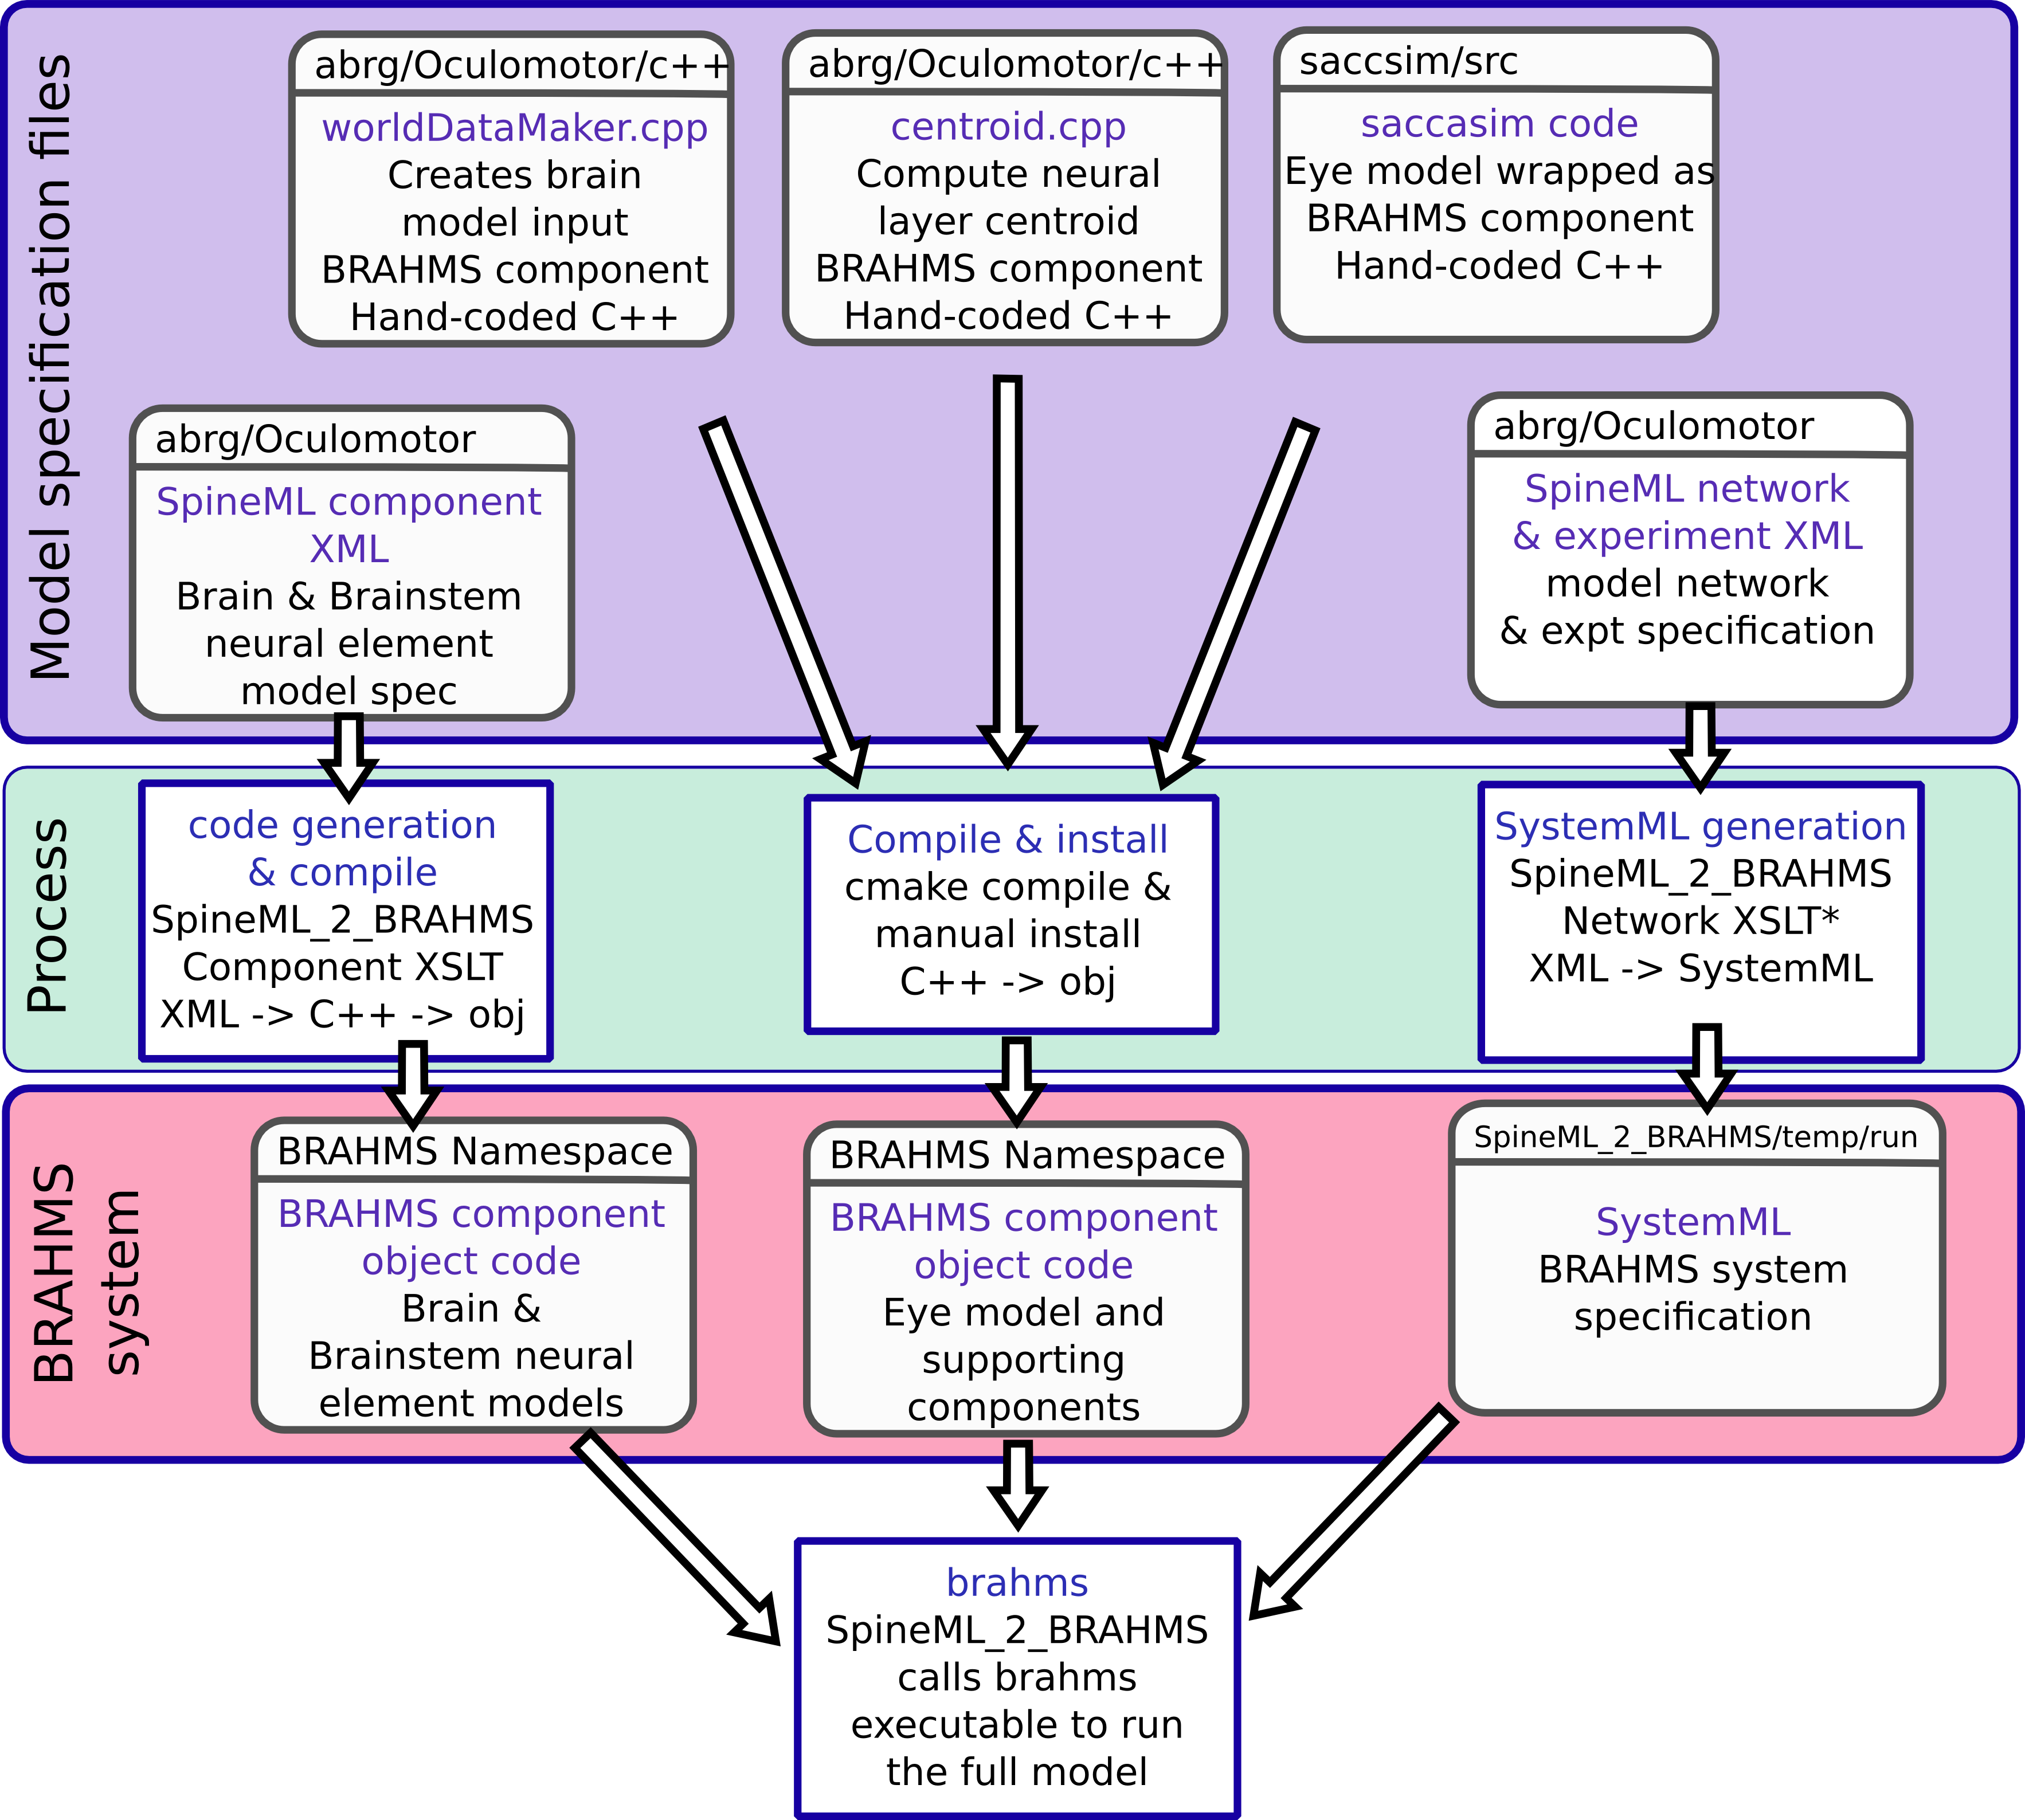
\includegraphics[width=0.9\textwidth]{./figures/model_framework.png}
\end{center}
\textbf{\refstepcounter{figure}\label{model_framework} Figure \arabic{figure}.}
{ The model framework. The model is specified using a combination of
declarative XML files and hand-coded C++. These original model
specifications are shown within the blue box. b) The green box shows
the processes which are applied to the model specification to produce
the BRAHMS system. Most of the process is defined within the scripts
which make up \stob, but the hand-written components must be manually
compiled and installed within the BRAHMS Namespace, allowing the
BRAHMS executable to locate them at runtime. c) The red box shows the
resulting BRAHMS system ready to be executed by the BRAHMS
executable. In practice, this call is made by \stob.}
\end{figure}

\begin{figure}[htb!]
\begin{center}
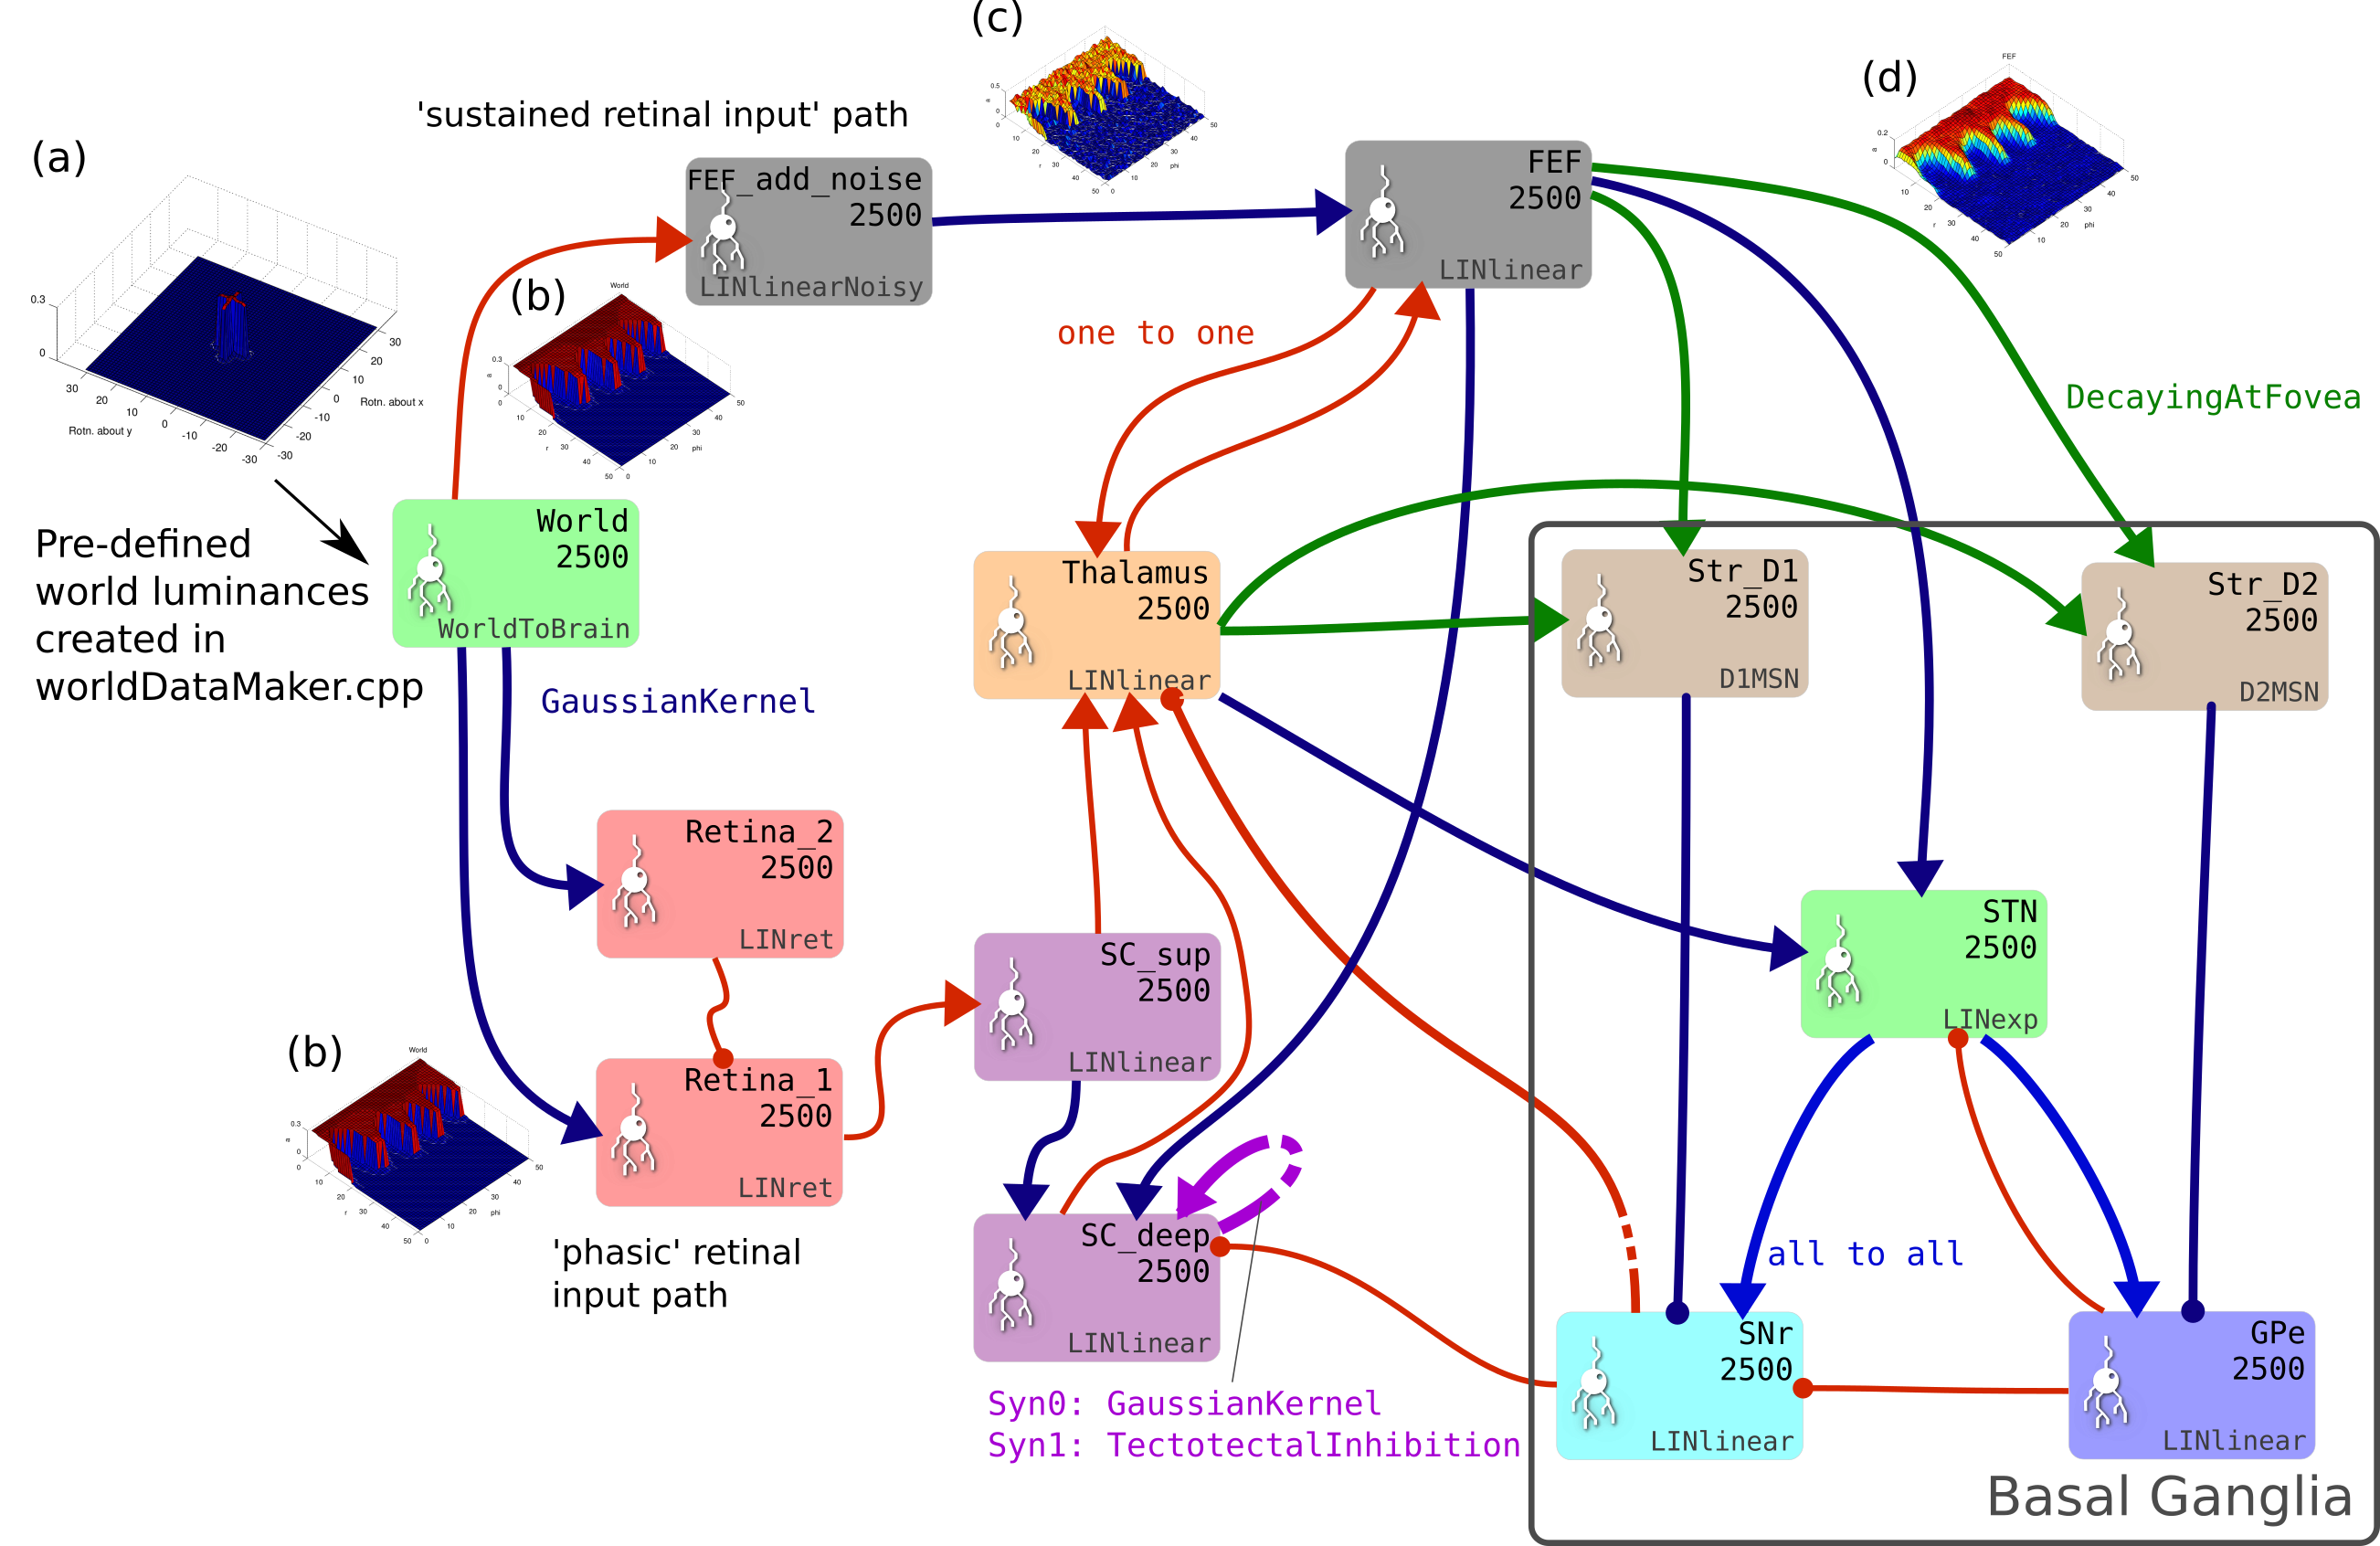
\includegraphics[width=0.9\textwidth]{./figures/Brain_Model.png}
\end{center}
\textbf{\refstepcounter{figure}\label{brain_model} Figure \arabic{figure}.}
{ The brain model. This is the SpineCreator `network layer' view of
the model. Each box represents a neural population with 2500 elements,
arranged in a 50$\times$50 grid. The SpineML component name is printed
on the bottom right corner of each population box and the population
name is at the top. The overall connectivity between populations is
represented by the projection arrows with the colour indicating the
connectivity scheme (one-to-one connections are red, Gaussian kernel
connections are dark blue and so on). Excitatory connections have
arrowheads and inhibitory connections have circles, although for
details of the behaviour of the connections, the weight-update and
post-synapse components must be studied. Briefly, the model comprises
a \e{World} population, into which a retinotopically organised view of
the world is introduced. This information is passed into cortical
populations (FEF) and subcortical populations (SC) via a simple model
of the retina. These feed a cortico-thalamo-basal ganglia loop, which
selects which region of the deep layer of superior colliculus should
be disinhibited, allowing activity to build up therein. The five
populations comprising the basal ganglia are enclosed in a grey
outline. Note that substantia nigra pars compacta is not modelled
here, instead the level of dopamine in the striatum is set via a
parameter in the Str\_D1 and Str\_D2 populations}
\end{figure}

\begin{figure}[htb!]
\begin{center}
\includegraphics[width=0.9\textwidth]{./figures/mapping.png}
\end{center}
\textbf{\refstepcounter{figure}\label{fig:mapping} Figure \arabic{figure}.}
{ Representative mapping from eye's frame of reference in Cartesian
co-ordinates to retinotopic co-ordinates. (a) The mapping of
luminances in the eye's frame of reference. The world input is
pre-defined by a JSON configuration file. Luminance position, size and
shape can be defined in this file, along with the times at which
luminances appear and disappear. The worldDataMaker.cpp code computes
the locations of the luminances in the eye's frame of reference, given
its rotational state. It also computes a 2D Gaussian convolution of
the luminances. Here, there are two cross shaped luminances spanning
10\dg, one of value 0.8 at the fixation point (0,0) and one of value
0.5 at a peripheral position (0,-12\dg). Note that these crosses have
the same `bar width' of 2\dg~as the crosses used in the simulations,
but their span of 10\dg~is greater than the 6\dg~used in the
simulations, to make these images clearer. (b) The locations of the
luminances in the eye's frame of reference are then converted into
retinotopic co-ordinates, with centrally located luminances being
represented at low values of $r$ and more peripheral luminances having
higher values of $r$. $\phi$ encodes rotational angle: 1 and 50 encode
upward movement; 13 is left; 25 is down; 37 is right. The output of
the World component is fed into FEF\_add\_noise and into the retinal
neuron populations. The colour map makes it possible to distinguish
between the two crosses. (c) The FEF\_add\_noise populations adds a
level of noise to the signal representing processing of the signal in
visual cortex. (d) A Gaussian projection from FEF\_add\_noise to FEF
further blurs the activity in FEF. FEF is the input to the basal
ganglia and one input to superior colliculus.}
\end{figure}

\begin{figure}[htb!]
\begin{center}
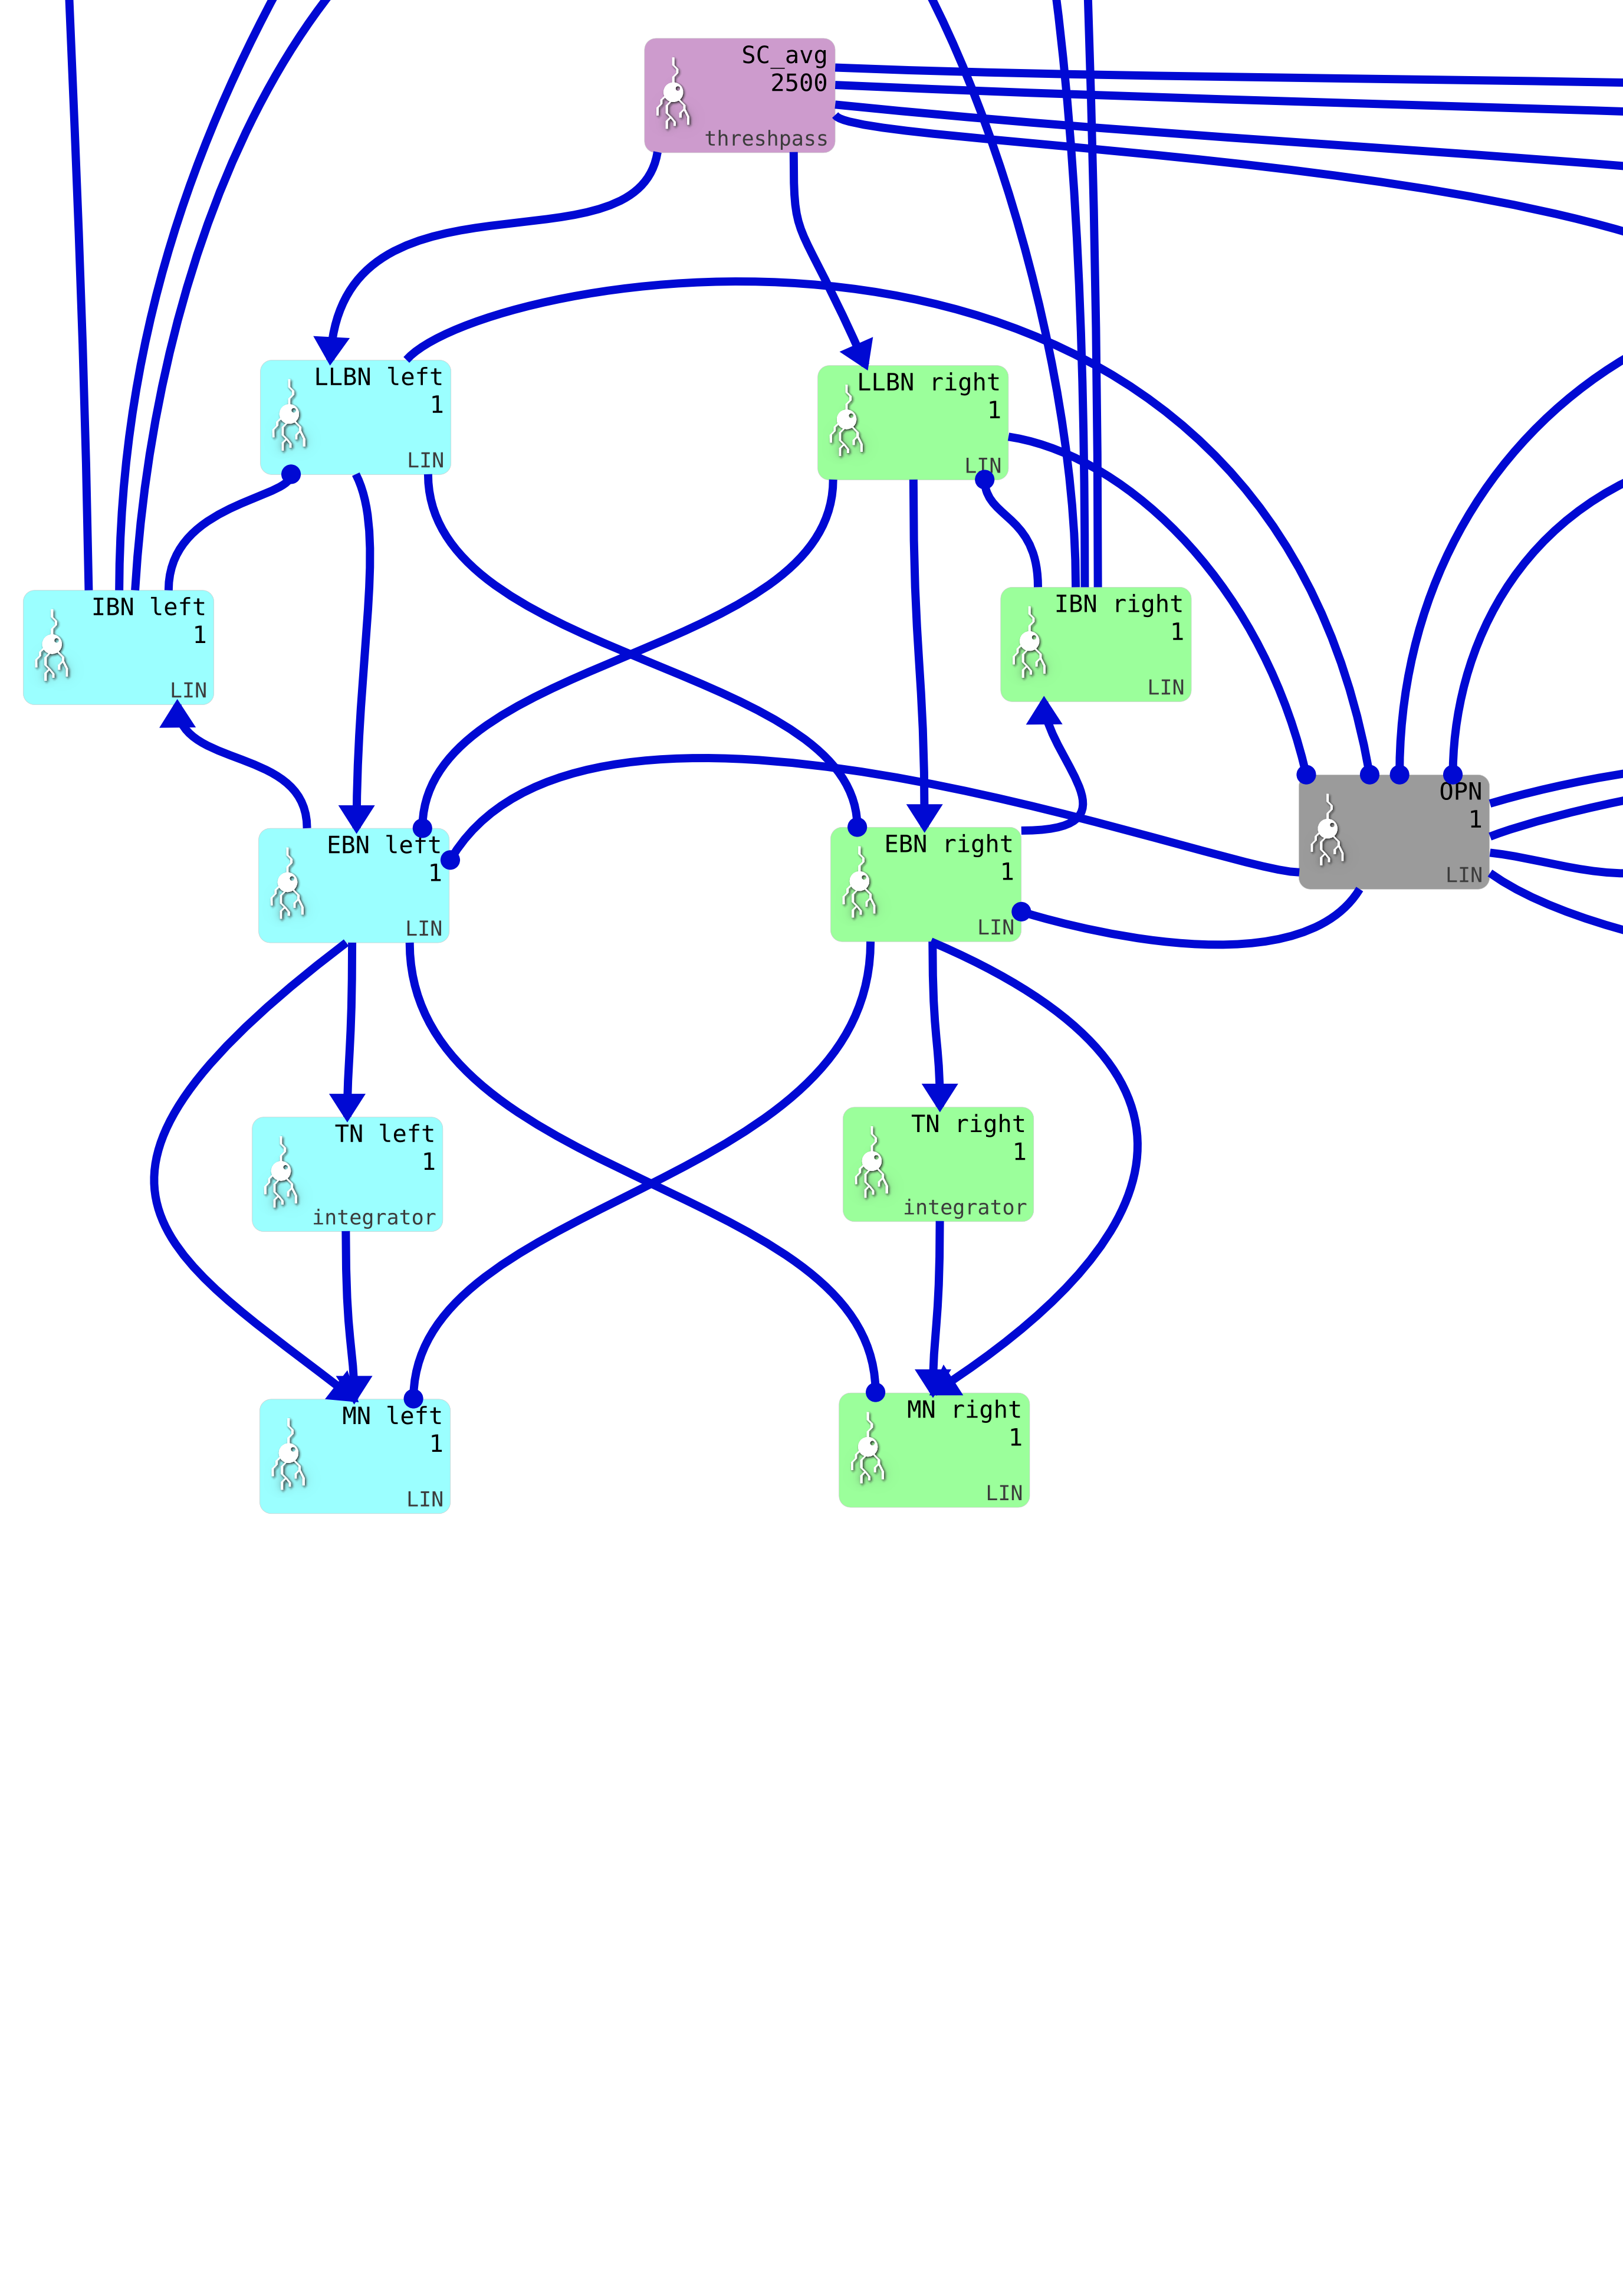
\includegraphics[width=0.5\textwidth]{./figures/Brain_Stem_1channel.png}
\end{center}
\textbf{\refstepcounter{figure}\label{sbg} Figure \arabic{figure}.}
{ One pair of channels of the saccadic burst generator (SBG) for left
(cyan) or right (green) movements. Collicular activity in SC\_avg
excites the channels via SBG weight maps. Each box represents a neural
population and shows the population name, the number of neural
elements (here 2500 or 1) and the SpineML component name; \e{LIN} for
Leaky integrator or \e{integrator}. Key: LLBN: Long lead burst
neurons; IBN: Inhibitory burst neurons; OPN: Omnipause neurons; EBN:
Excitatory burst neurons; TN: Tonic neurons; MN: Motoneurons.}
\end{figure}

\begin{figure}[htb!]
\begin{center}
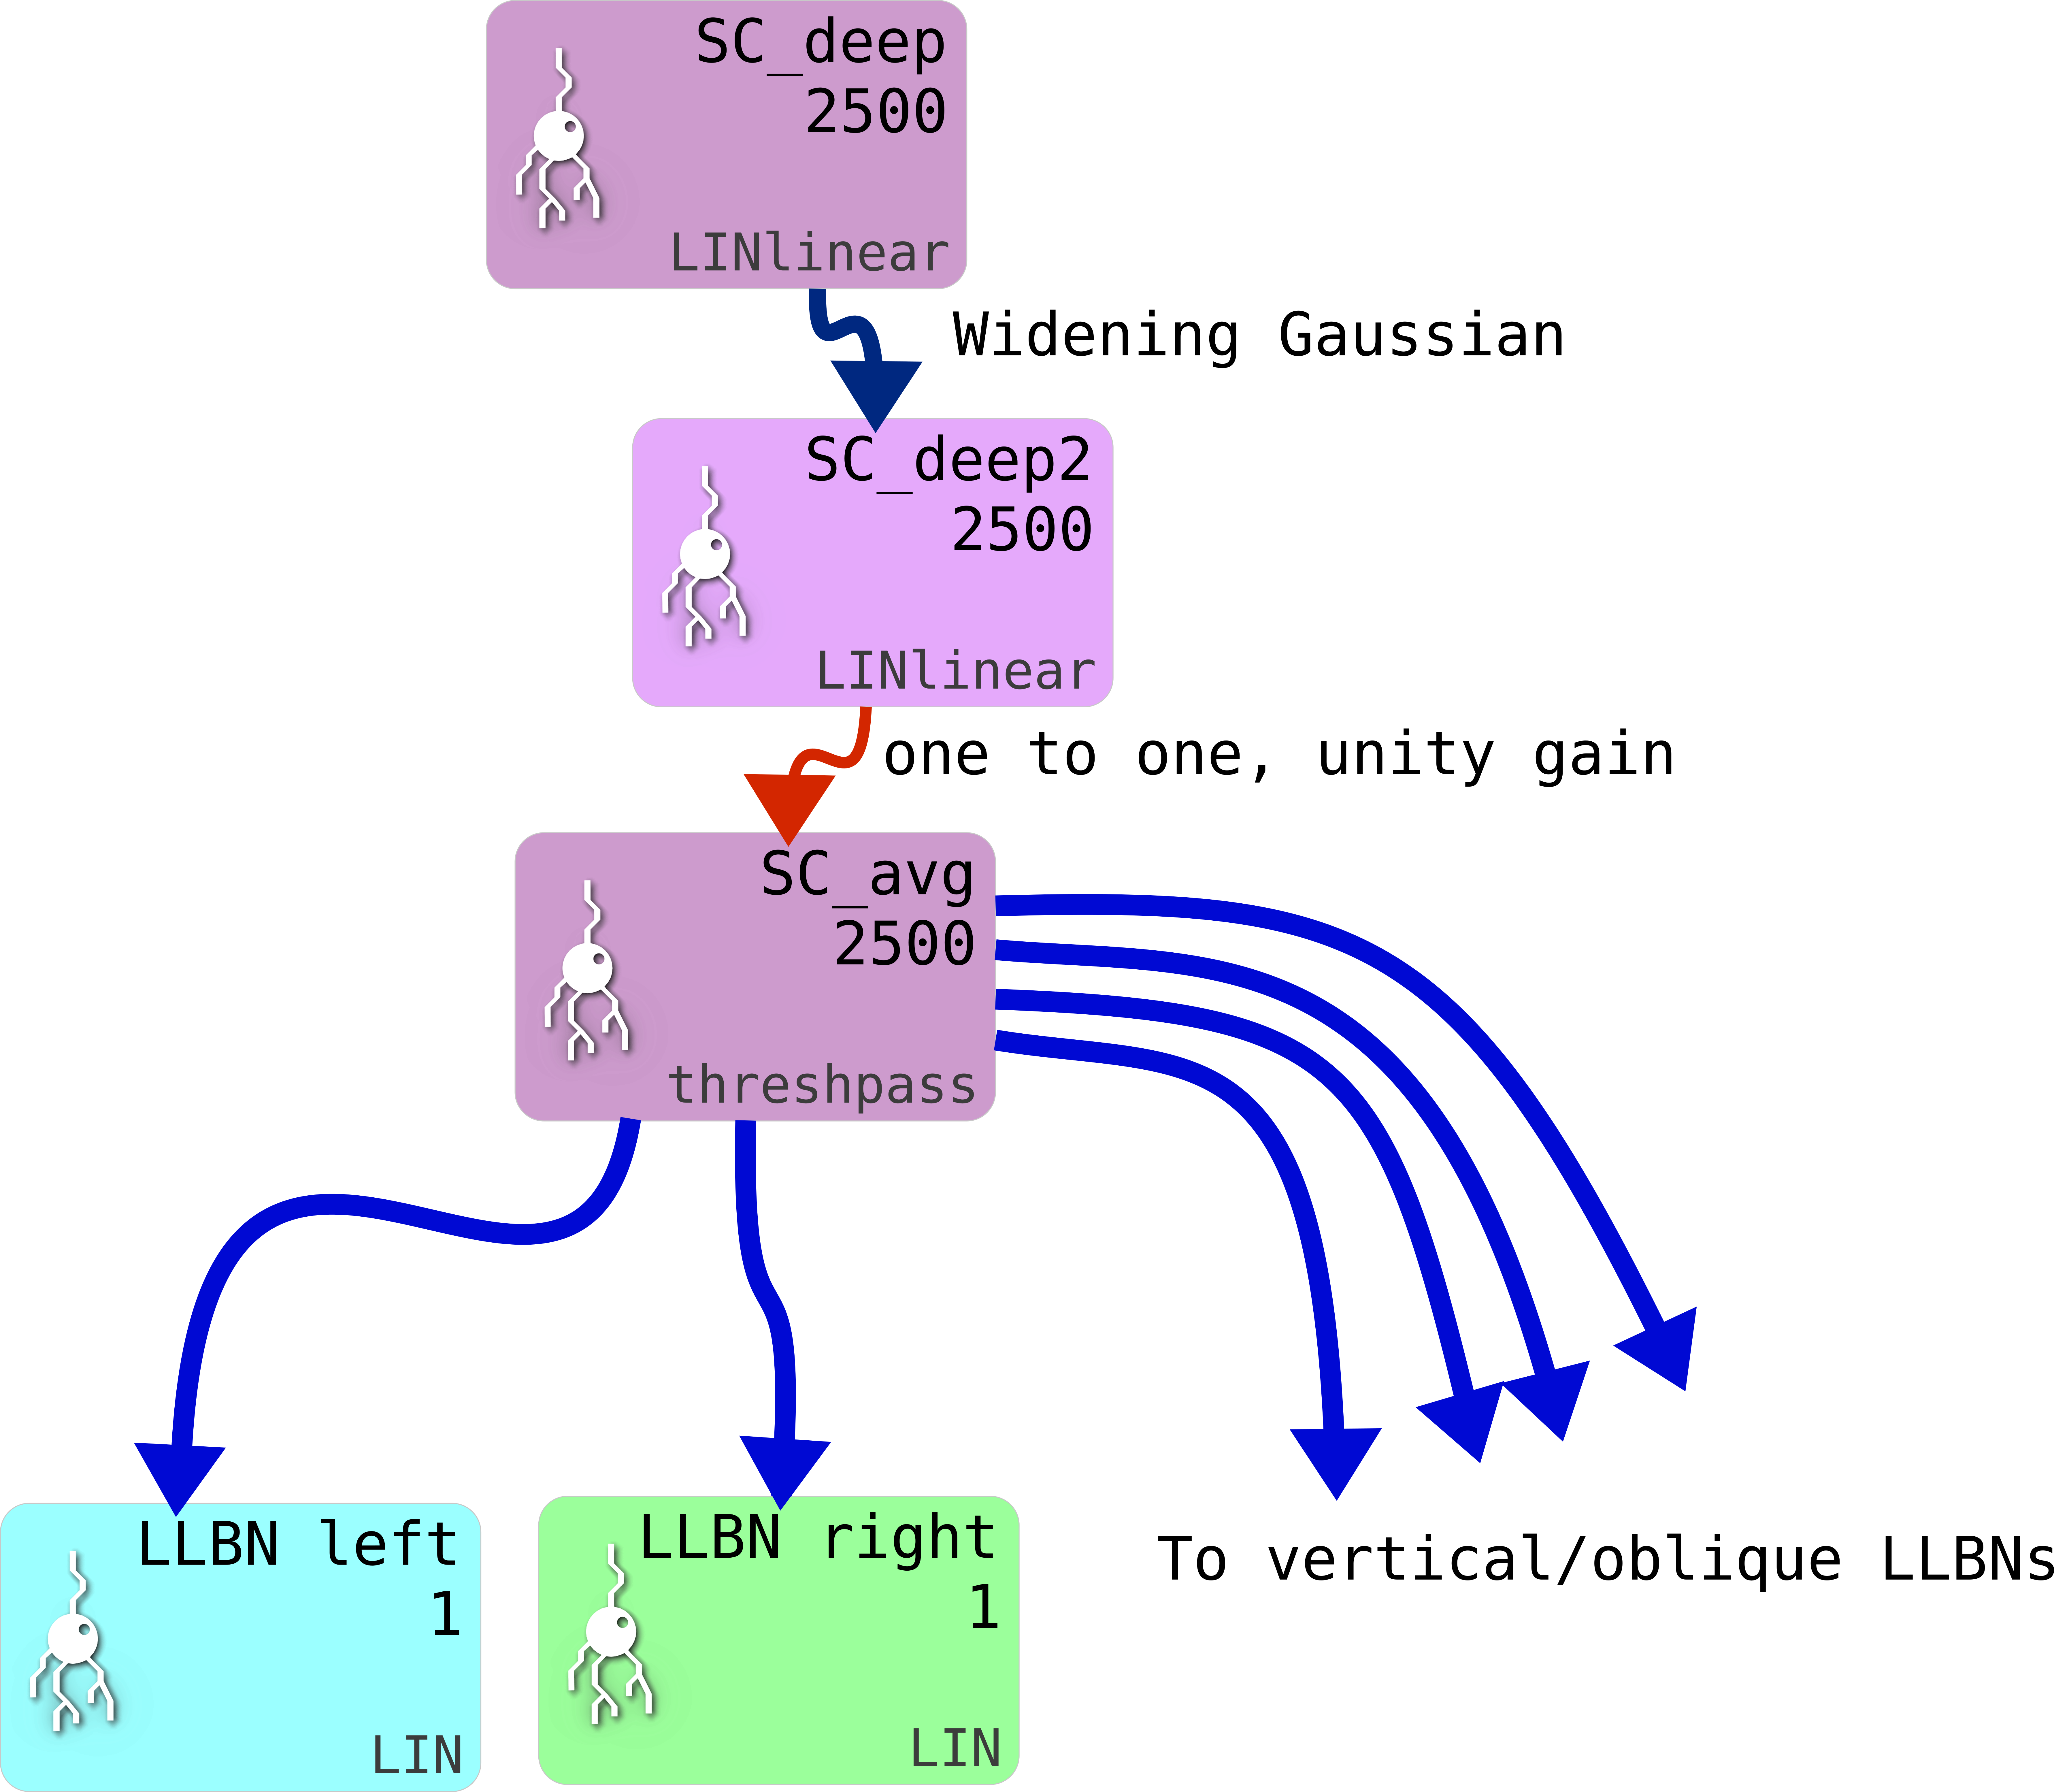
\includegraphics[width=0.5\textwidth]{./figures/SC_to_brainstem.png}
\end{center}
\textbf{\refstepcounter{figure}\label{scdeep} Figure \arabic{figure}.}
{ Showing the additional deep layer of superior colliculus (SC\_deep2)
and the output layer (SC\_avg, named for the fact that in an earlier
version of the model, it received the output of the centroid of
SC\_deep).  The widening Gaussian projection is shown as the arrow
between SC\_deep and SC\_deep2.}
\end{figure}

\begin{figure}[htb!]
\begin{center}
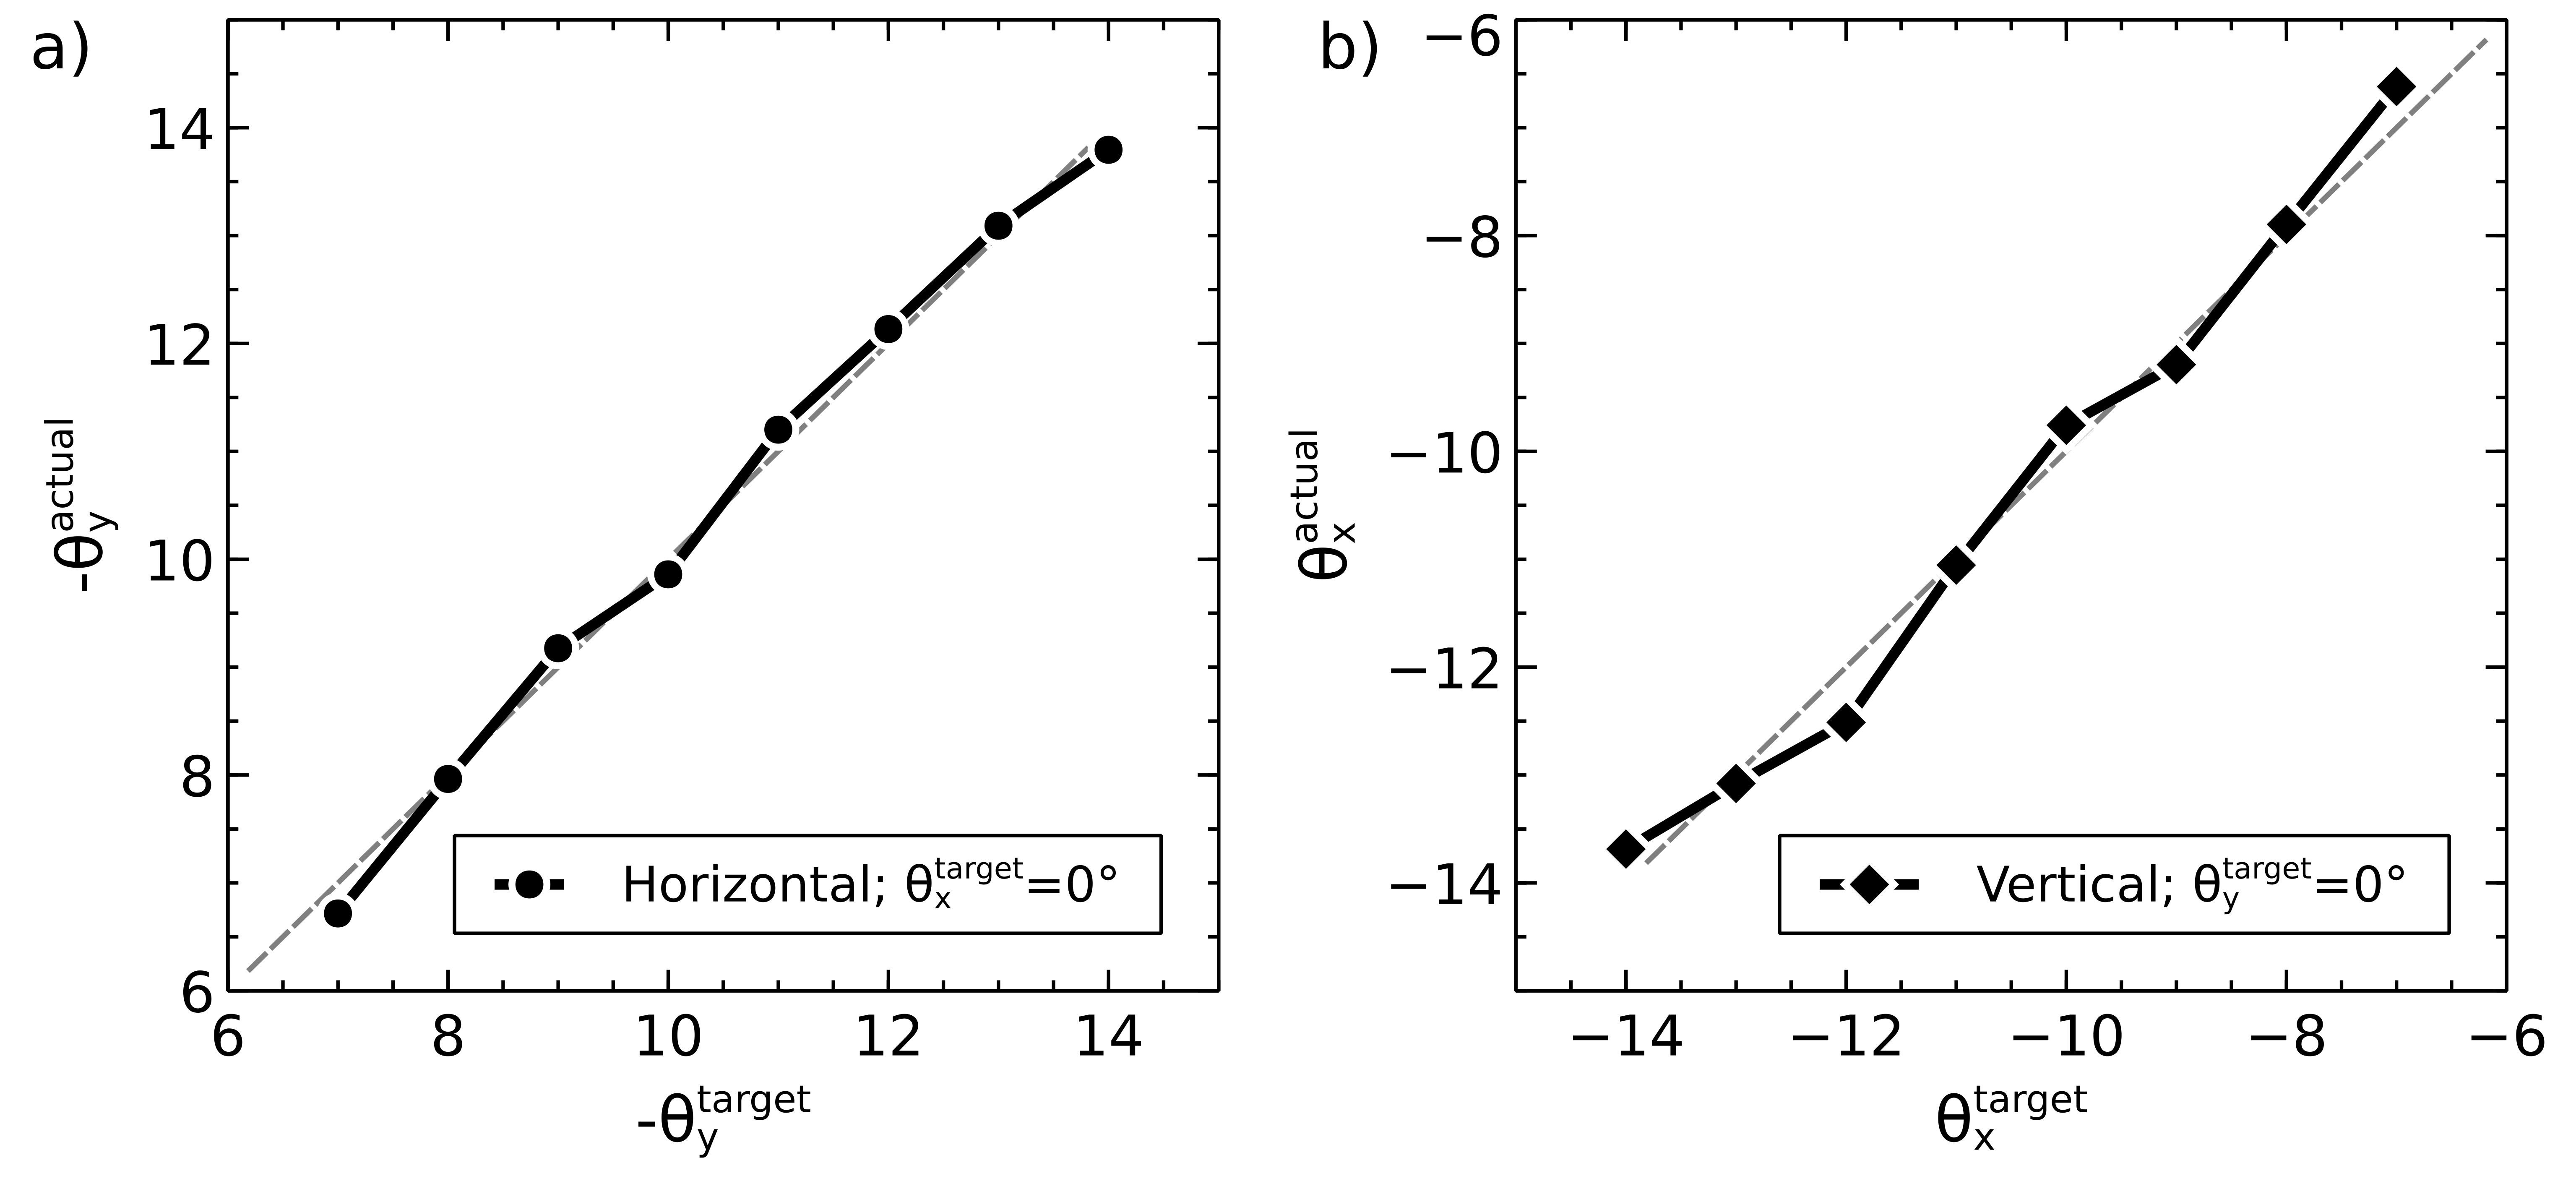
\includegraphics[width=0.8\textwidth]{./figures/sacc_vs_targetpos.png}
\end{center}
\textbf{\refstepcounter{figure}\label{sacc_vs_targ} Figure \arabic{figure}.}
{ Accuracy at different target eccentricities for fixation luminance
0.2 and target luminance 0.3.}
\end{figure}

\begin{figure}[htb!]
\begin{center}
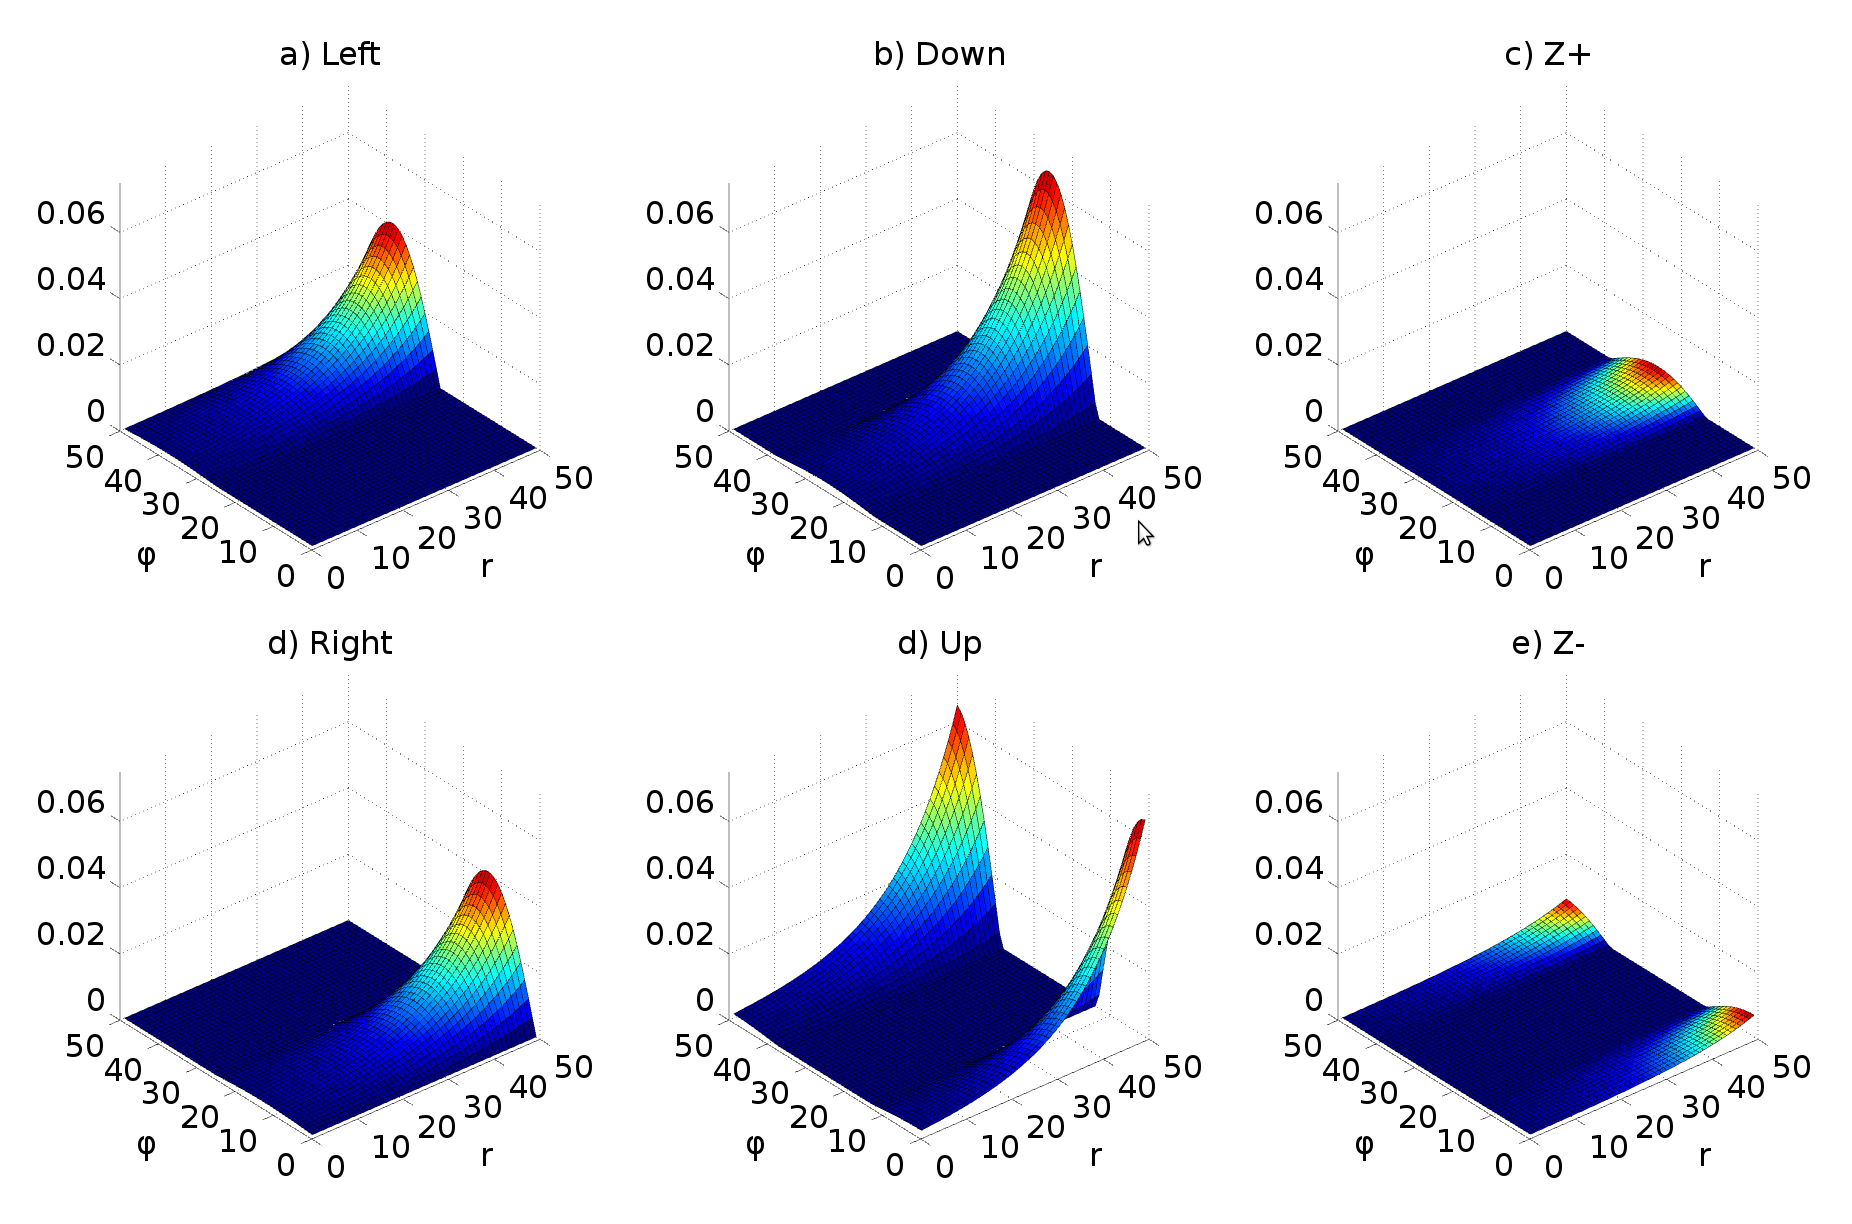
\includegraphics[width=\textwidth]{./figures/weightmaps.png}
\end{center}
\textbf{\refstepcounter{figure}\label{weightmaps} Figure \arabic{figure}.}
{ Weight maps for the connections between the output layer of superior
colliculus and the six long lead burst neurons of the saccadic burst
generator model. Each map increases exponentially with increasing $r$,
multiplied by cosine($\phi$) about its `active' axis.}
\end{figure}

\begin{figure}[htb!]
\begin{center}
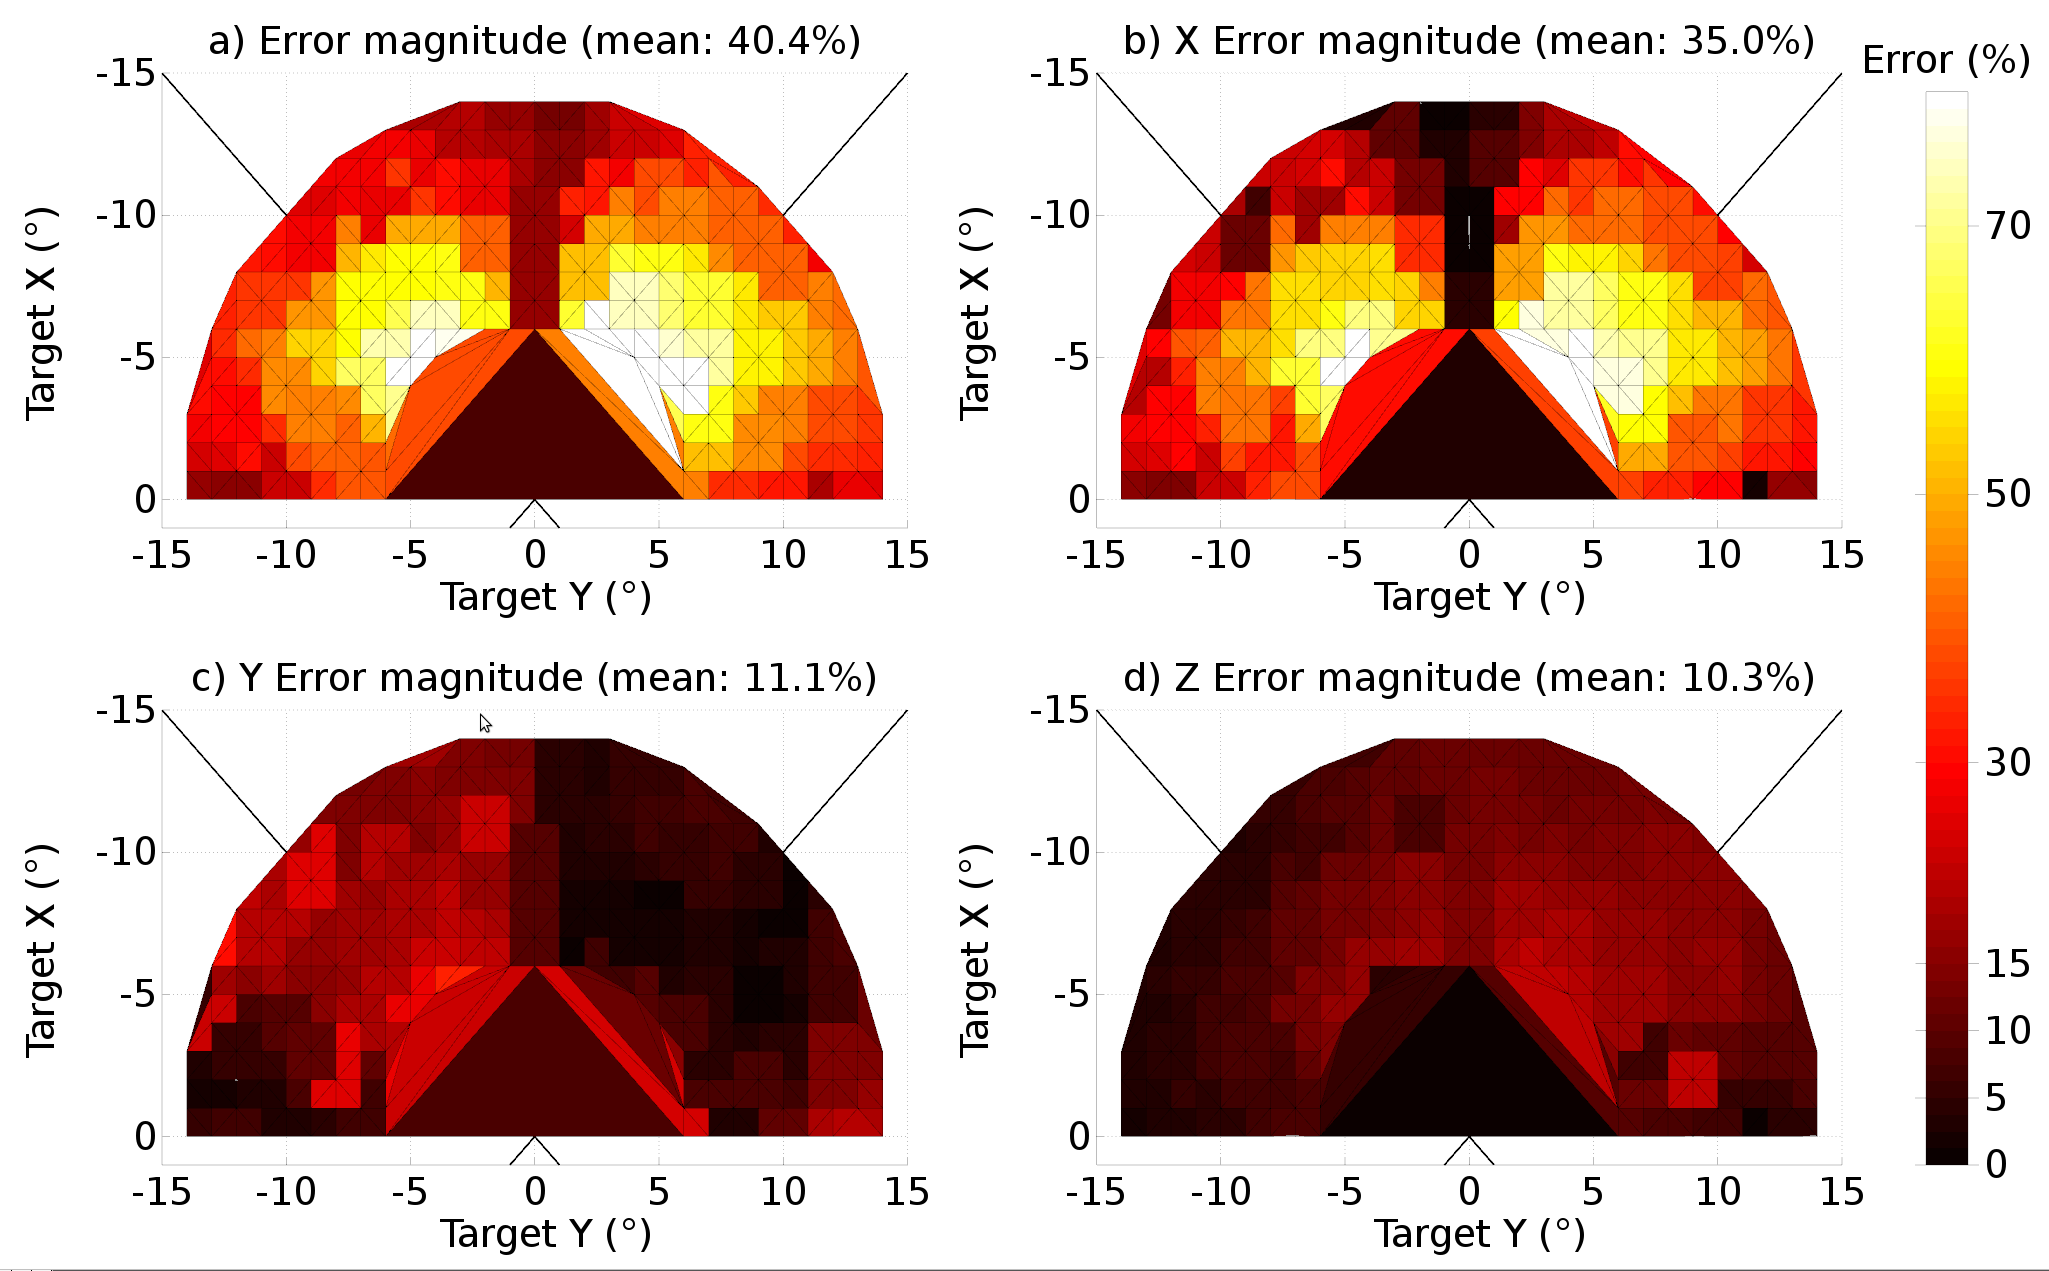
\includegraphics[width=0.95\textwidth]{./figures/errorsurface_TModel3.png}
\end{center}
\textbf{\refstepcounter{figure}\label{errorsurfaceTM3} Figure \arabic{figure}.}
{ The end-point error surface for the original, na\"ive model
(TModel3). a) The ratio of the magnitudes of the total error vector
and the target vector, expressed as a percentage. b) The ratio of the
magnitude of the $x$ component of the error vector to the magnitude of
the target vector, expressed as a percentage. c) As (b) but for the
$y$ component. d) As (b), for $z$ component. All colour maps are shown
with the same scale. The target rotations, $\theta_{x}^t$ and
$\theta_{y}^t$ are denoted `Target X' and `Target Y' in the figure.}
\end{figure}

\begin{figure}[htb!]
\begin{center}
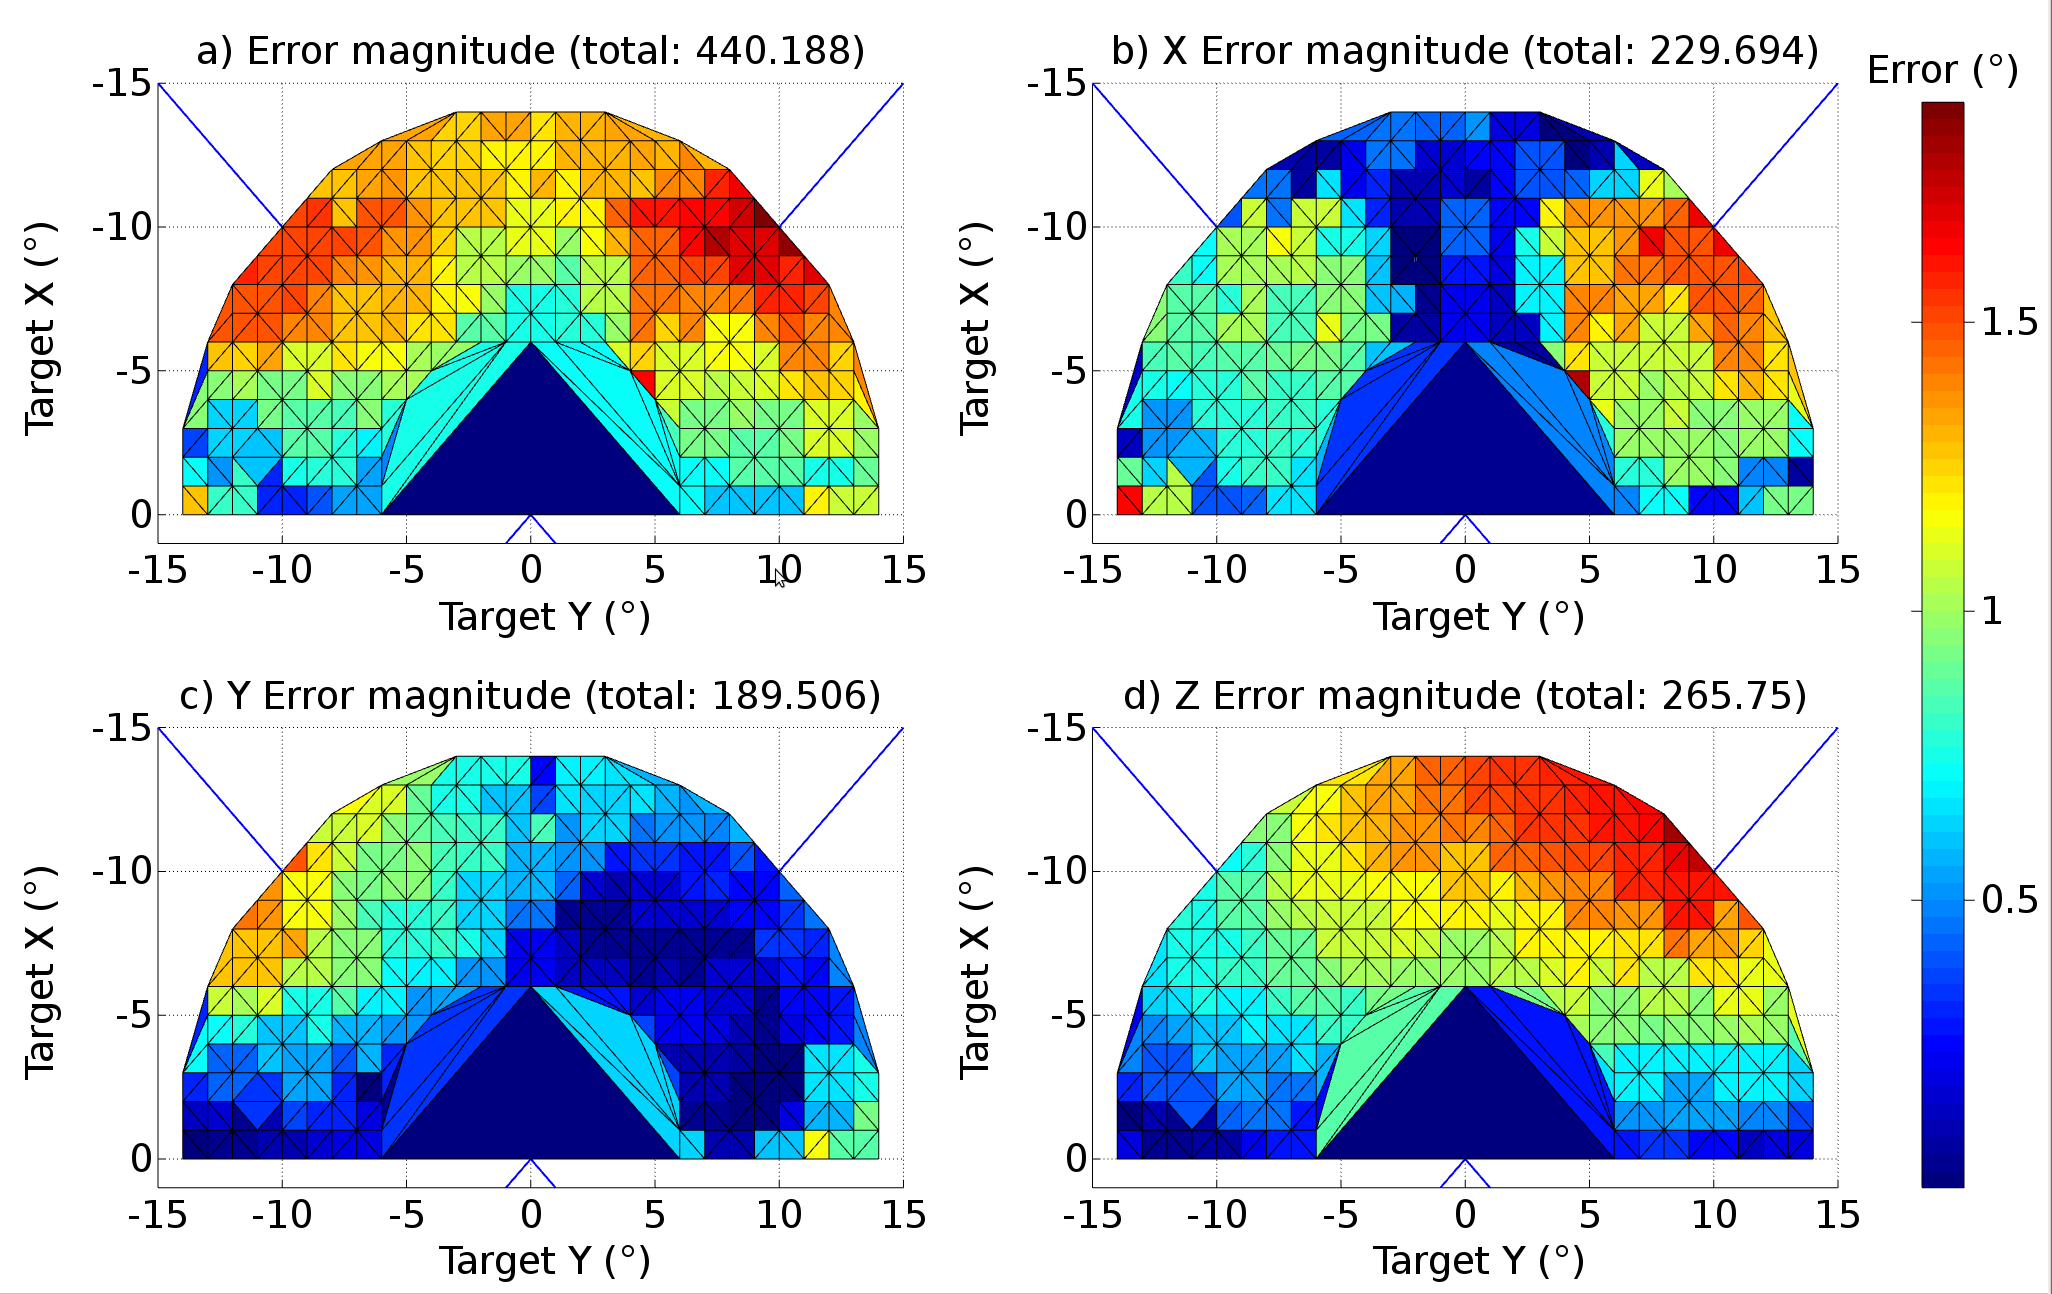
\includegraphics[width=0.95\textwidth]{./figures/errorsurface.png}
\end{center}
\textbf{\refstepcounter{figure}\label{errorsurface} Figure \arabic{figure}.}
{ The end-point error surface for the model in which a widening
projection field was added to the model of the superior colliculus. a)
The ratio of the magnitudes of the total error vector and the target
vector, expressed as a percentage. b) The ratio of the magnitude of
the $x$ component of the error vector to the magnitude of the target
vector, expressed as a percentage. c) As (b) but for the $y$
component. d) As (b), for $z$ component. All colour maps are shown
with the same scale. The target rotations, $\theta_{x}^t$ and
$\theta_{y}^t$ are denoted `Target X' and `Target Y' in the figure.
Note that the range of the colour scale is 0 to 20\%, a much smaller
range than the range in Fig~\ref{errorsurfaceTM3}.}
\end{figure}

\begin{figure}[htb!]
\begin{center}
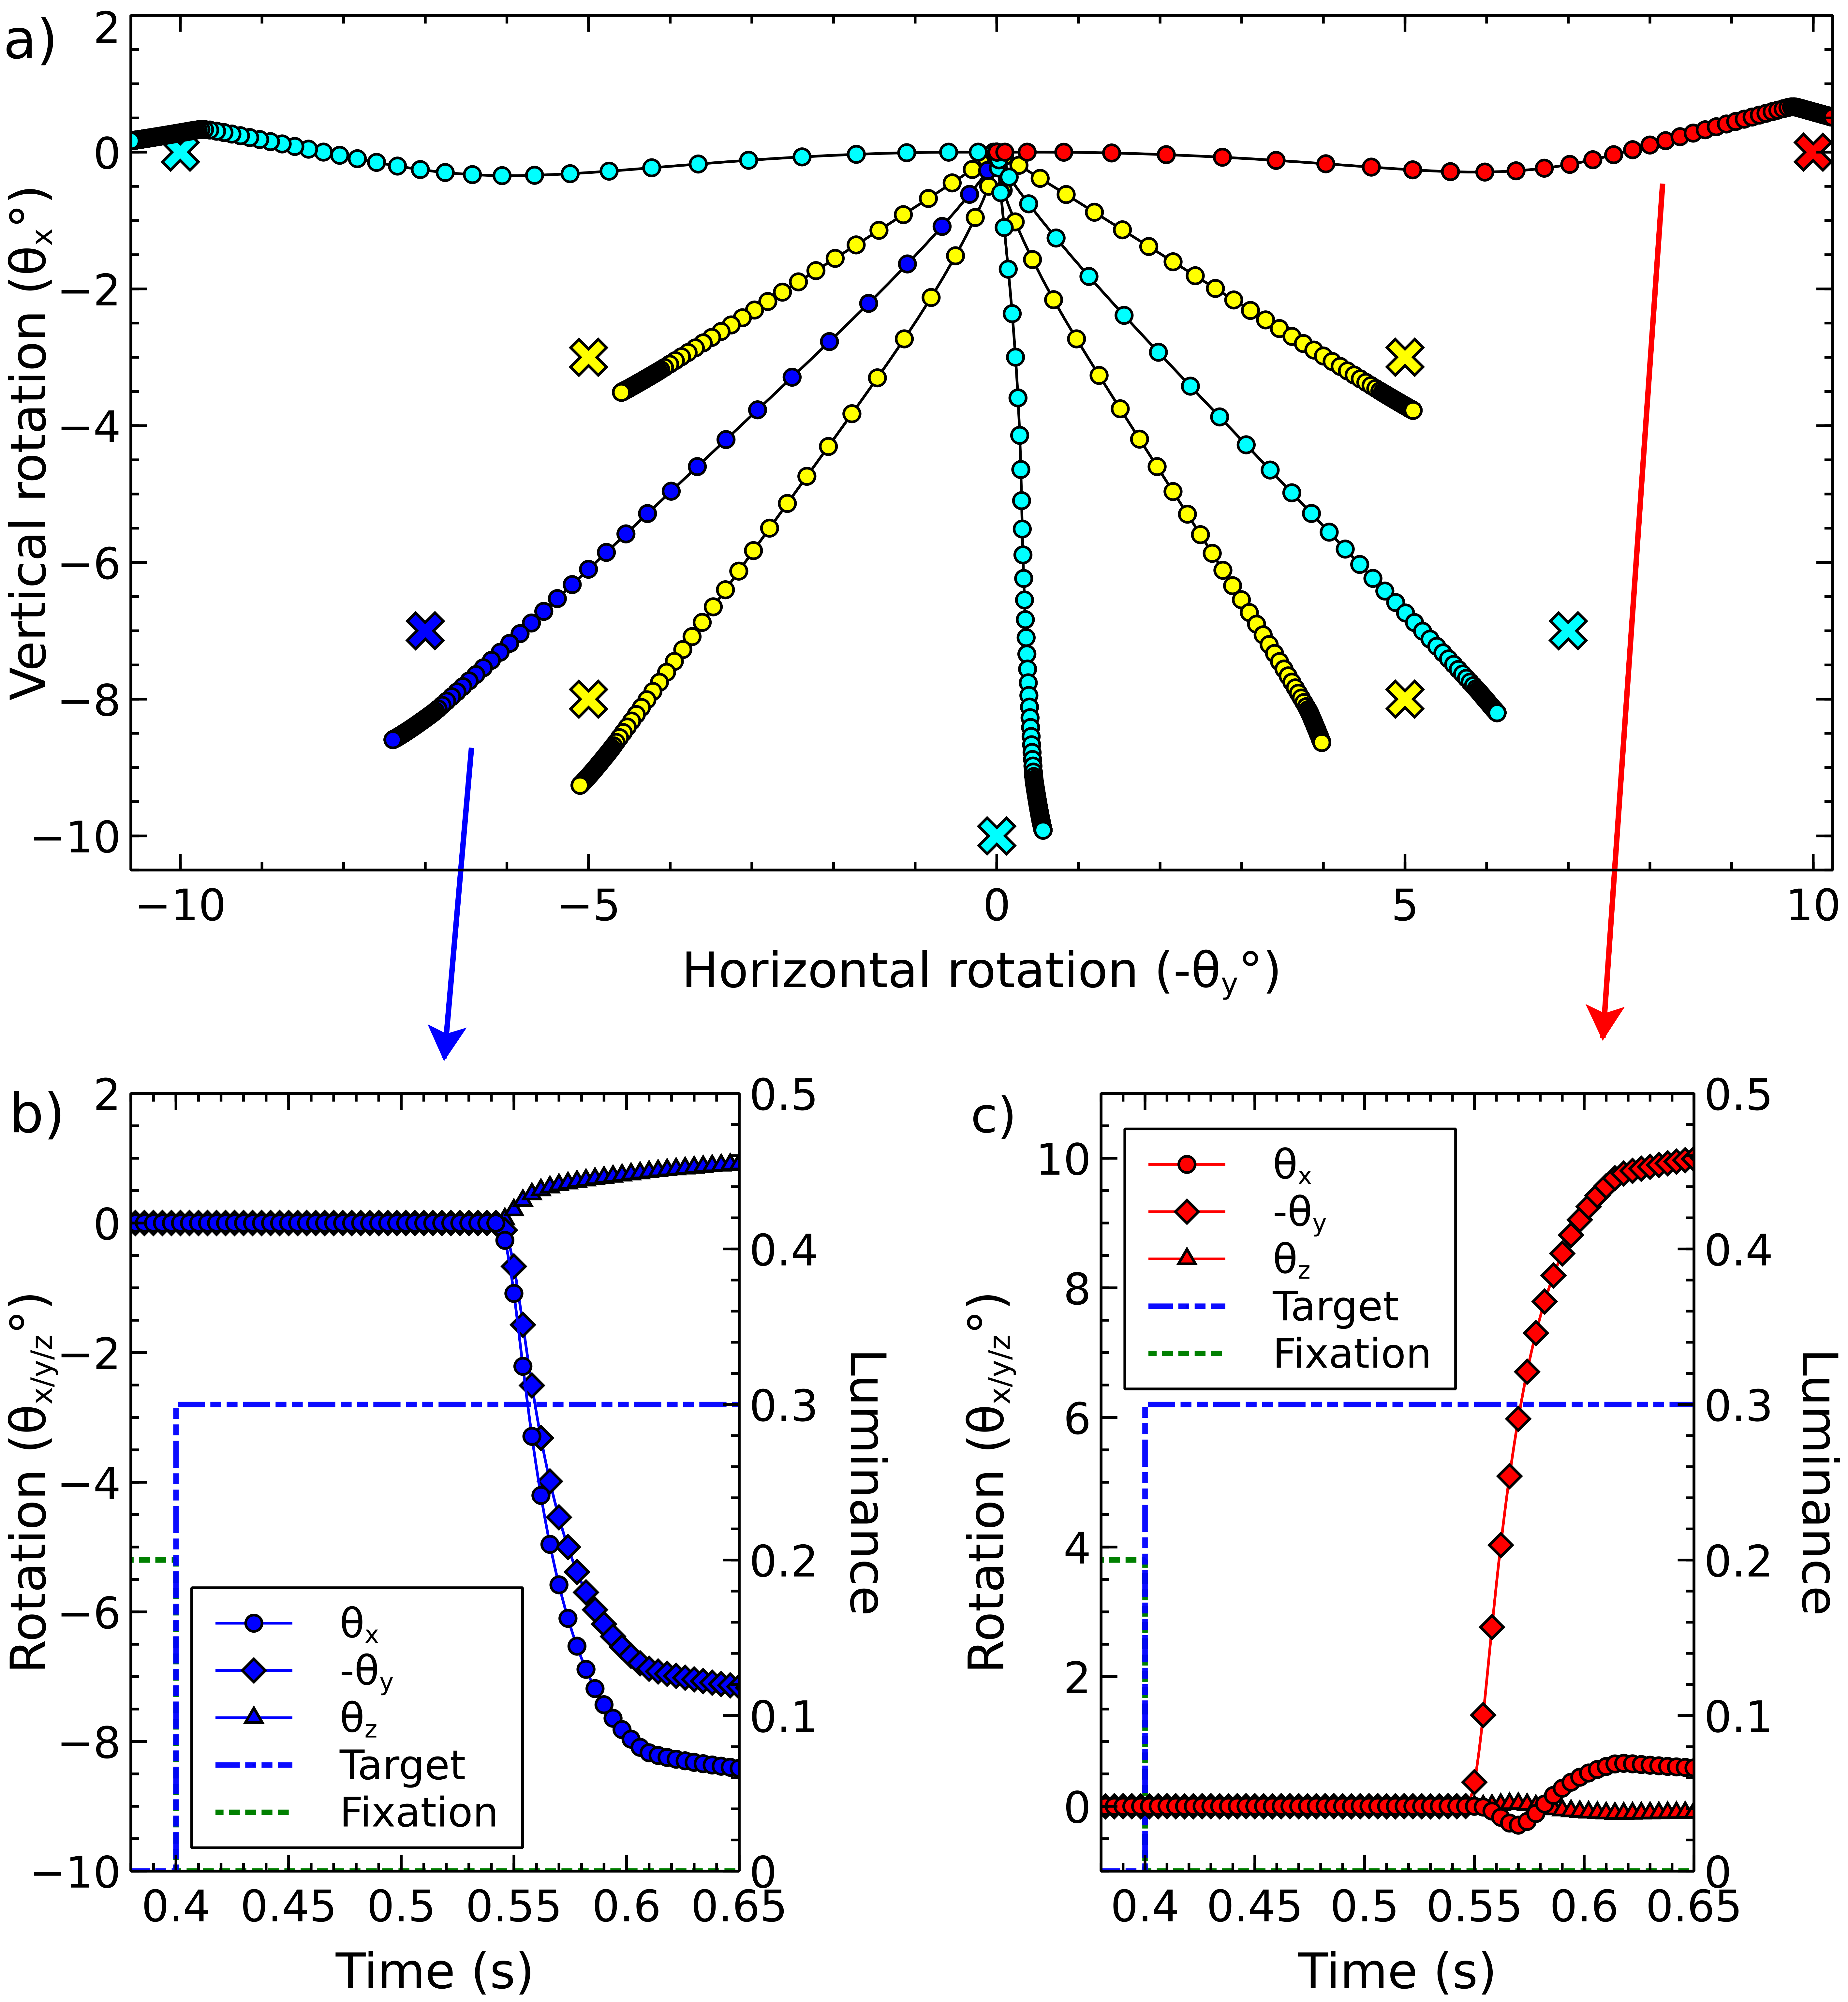
\includegraphics[width=0.8\textwidth]{./figures/outmany.png}
\end{center}
\textbf{\refstepcounter{figure}\label{outmany} Figure \arabic{figure}.}
{ Representative single saccades. a) Trajectories from 9 saccades to a
single target at 9 different locations. In each case, a fixation cross
luminance of magnitude 0.2 was displayed at (0,0), the start position
of the eye, until time 0.4~s. The target luminance, magnitude 0.3 was
illuminated at time 0.4~s. Trajectory shape is dependent on the target
position, and there is a variable amount of error in the end-points
achieved by the model. Colour is used in this diagram as an aid to
distinguishing different saccades and their targets; for a given
saccade, the target location is given by the cross of the same colour
closest to the end of the trajectory. b) The three rotational
components of the `blue' saccade, to target location (-7,-7). c) The
three rotational components of the `red' saccade, to target location
(0,-10).}
\end{figure}

\begin{figure}[htb!]
\begin{center}
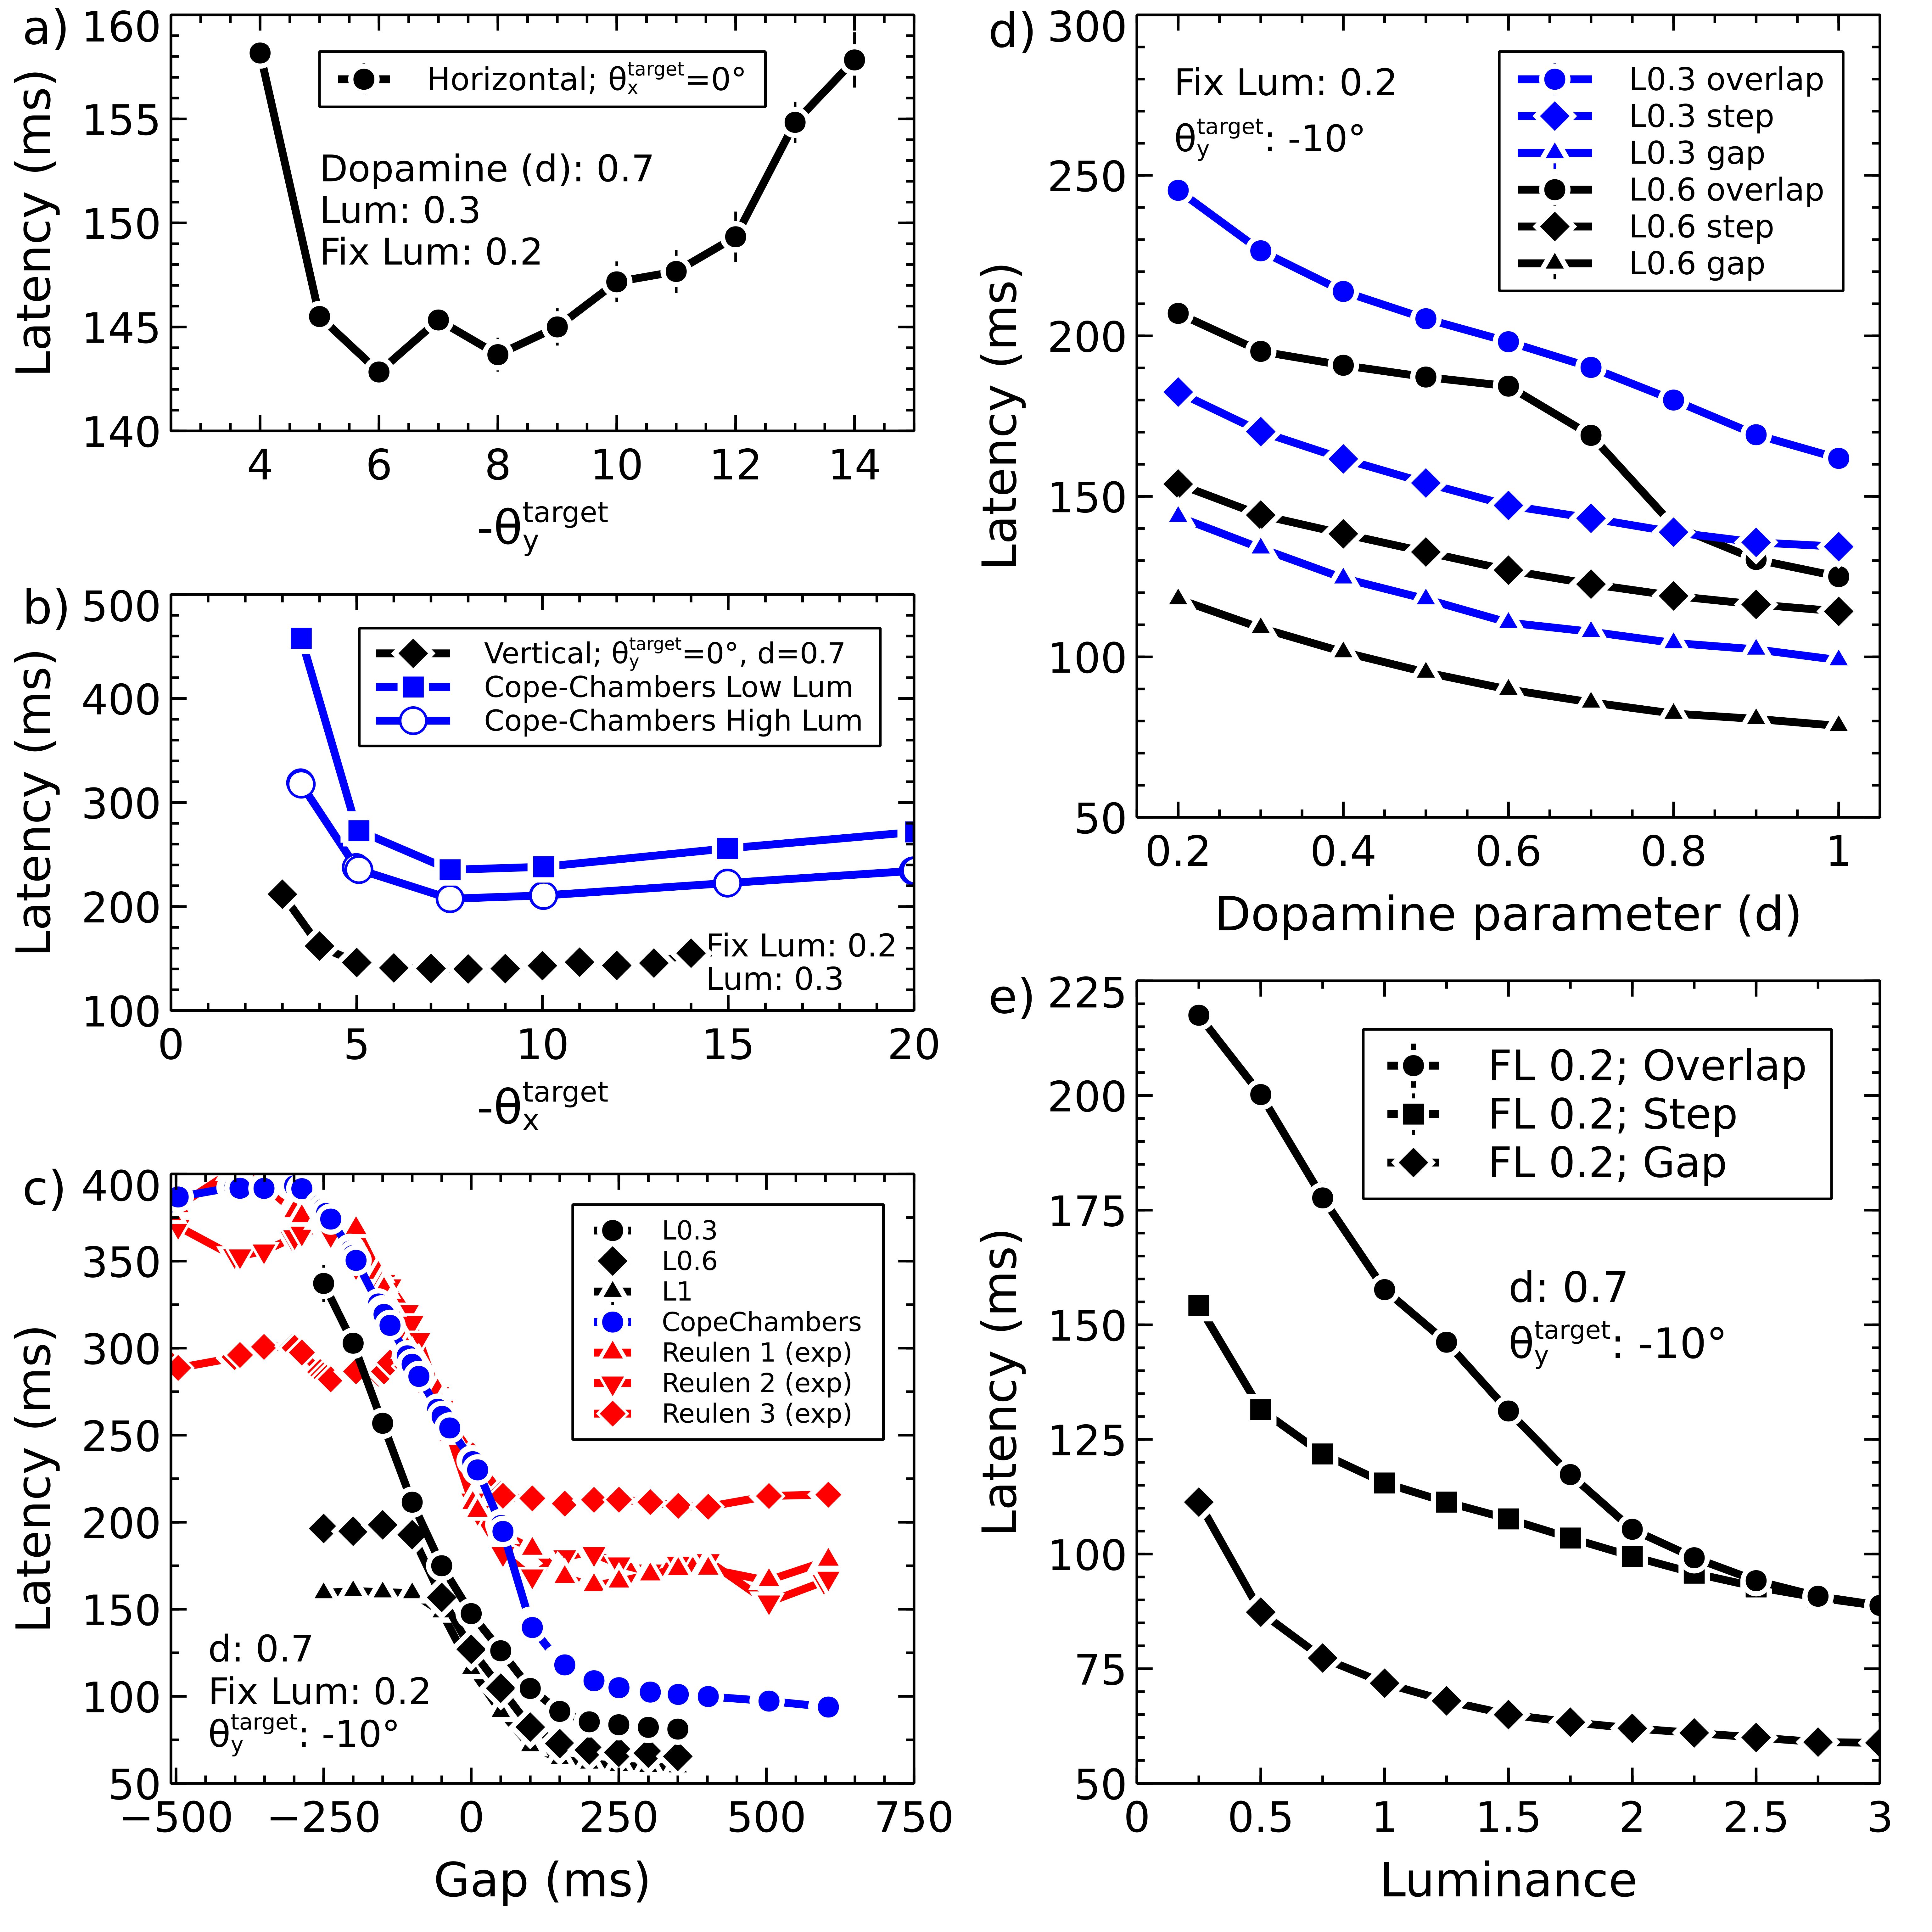
\includegraphics[width=0.8\textwidth]{./figures/lat_vs_everything.png}
\end{center}
\textbf{\refstepcounter{figure}\label{lat_vs_all} Figure \arabic{figure}.}
{ Exploring saccade latencies. a) Latency to first movement as a
function of target eccentricity for horizontal targets. b) Latency
vs. eccentricity for vertical targets. c) Latency vs. gap at three
different luminance values. d) The effect of the dopamine parameter on
saccade latencies in gap, step and overlap conditions, for two
different target luminances.  e) Saccade vs. luminance showing gradual
transition between reflexive and express behaviour.
%f) Saccade duration vs. saccade eccentricity for horizontal
%(rightwards), vertical (downwards) and 45\dg~oblique (down \& right) saccades.
}
\end{figure}

\begin{figure}[htb!]
\begin{center}
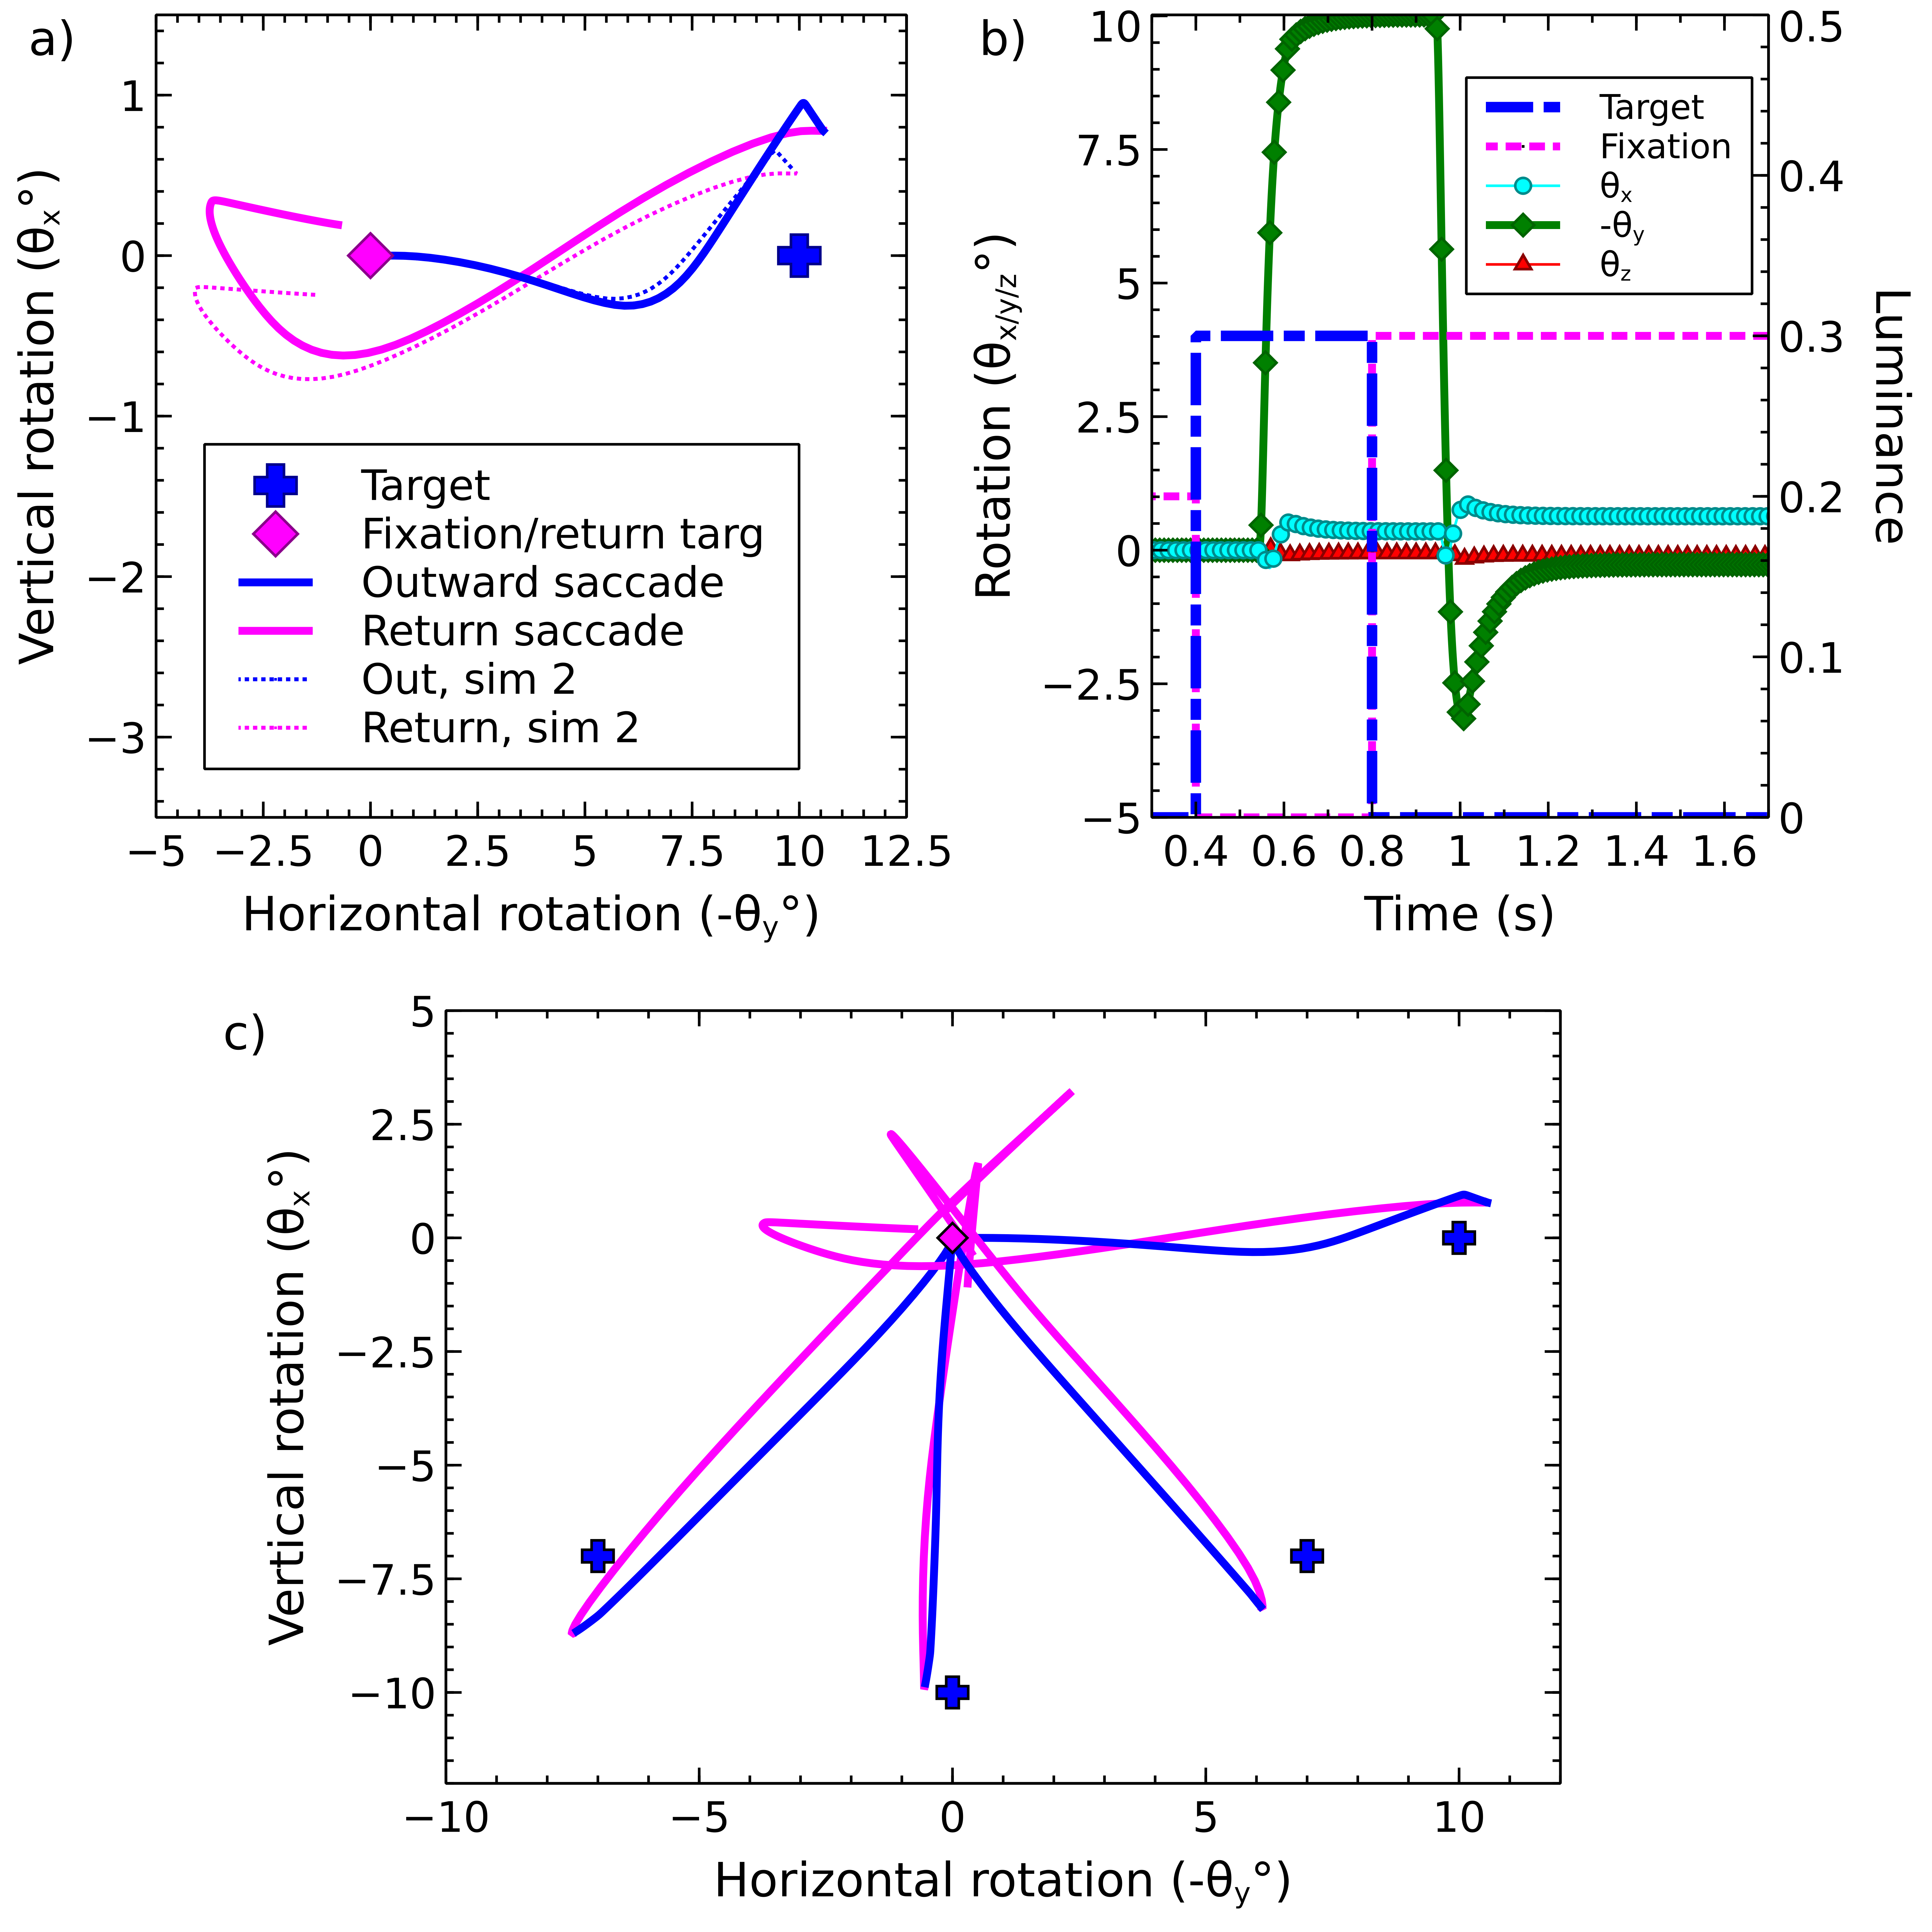
\includegraphics[width=0.8\textwidth]{./figures/outrtn.png}
\end{center}
\textbf{\refstepcounter{figure}\label{outrtn} Figure \arabic{figure}.}
{ There and back - a saccade to a target, followed by return to the
original fixation. a) Out and return saccade to a target at (0,-10\dg)
b) Rotational components of the saccade shown in (a). c) Outward and
return trajectories for the saccade shown in (a) alongside saccades to
three other targets.}
\end{figure}

\begin{figure}[htb!]
\begin{center}
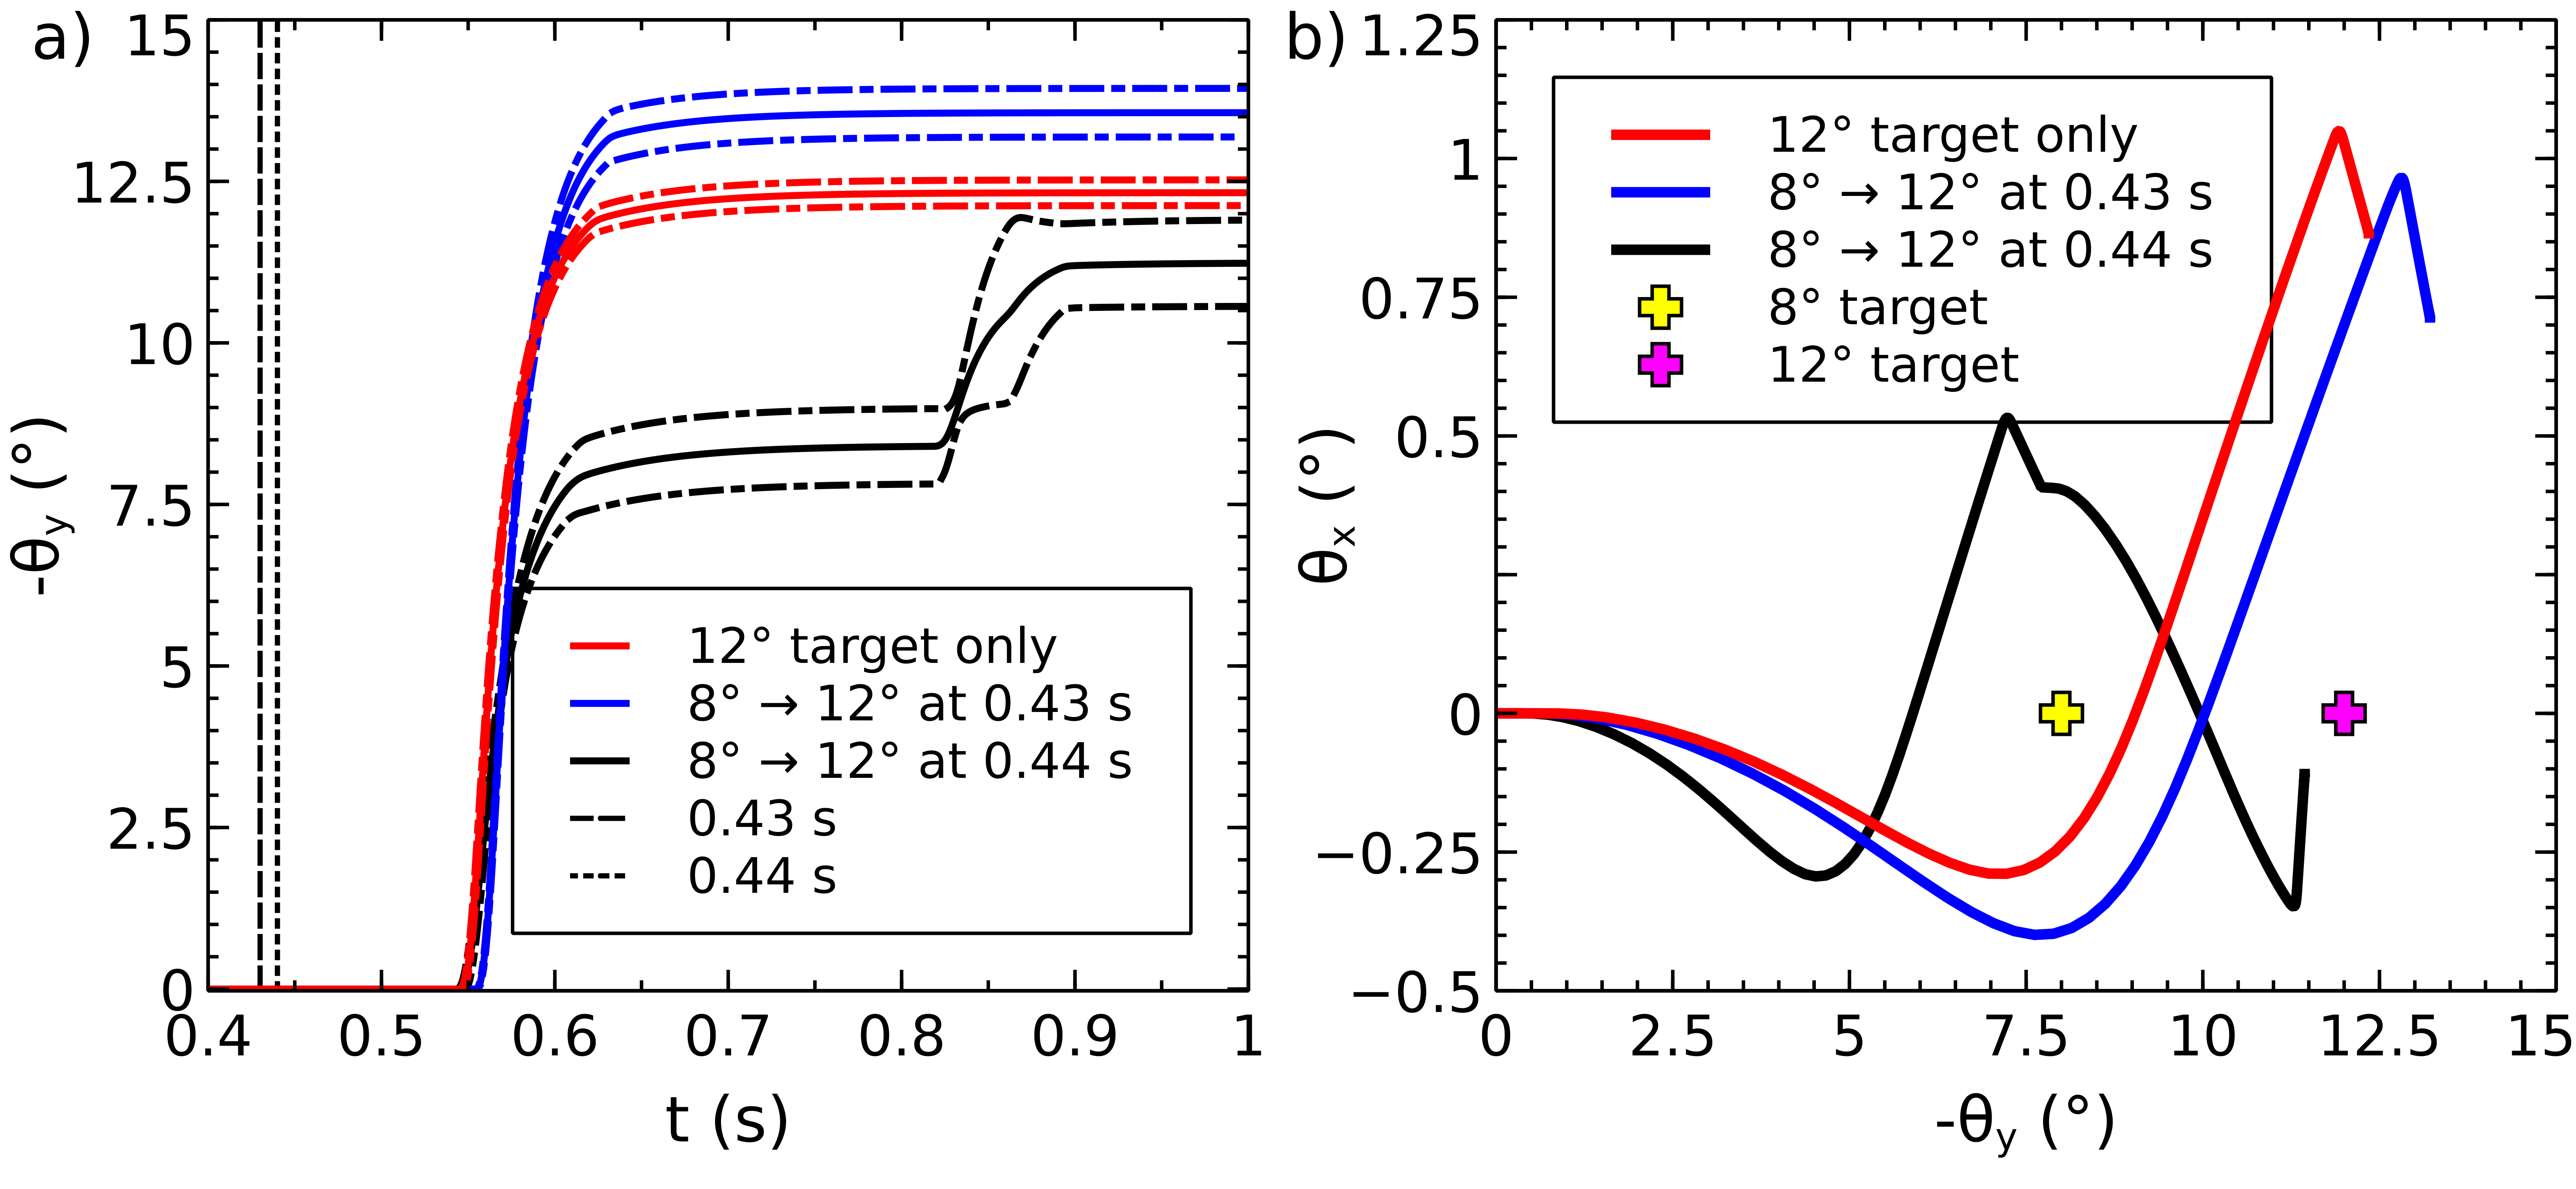
\includegraphics[width=0.8\textwidth]{./figures/doublesteps.png}
\end{center}
\textbf{\refstepcounter{figure}\label{doublesteps} Figure \arabic{figure}.}
{ Double steps. The effect of illuminating a first target at 8\dg~or
12\dg, followed by a second target at 12\dg~or 8\dg. a) Horizontal
rotation of the eye plotted vs.~time for a saccade to the 12\dg~target
only (red), and to an 8\dg~target at 0.4~s followed by a 12\dg~target
after 30~ms (blue) or 40~ms (black). The timings are indicated by
vertical lines. When the second target is presented up to 30~ms after
the initial target, the initial target has not had time to dominate
the output saccade and a saccade to a location close to the second
target is made. If the delay is 40~ms or more, the activity from the
initial target has time to cause a built up of actiivty in SC\_deep
and an initial saccade close to the first target is made, followed,
after a longer than usual latency period, with a second saccade closer
to the second target. In this graph, the mean of five separate
simulations is plotted along with $\pm$1 standard deviation around the
mean. b) The $\theta_{x}$/$\theta_{y}$ trajectories corresponding to
the data presented in (a).}
\end{figure}

\end{document}
